% !TEX root =  main.tex
\chapter{Constraints}
\label{ch: constraints}


This catalog aggregates constraints related to the management of VMs and
servers on hosting platforms. 
%
Previous chapters present key elements that may be impacted by a reconfiguration :
VM state and placement, server state, resource allocation.
%
The present chapter enumerates numerous constraints that are of a practical interest
for applications and datacenter administrators to express dependability or management
requirements such as performance, availability or security.
%
Such constraints may then be implemented in different VM managers to provide an initial
deployment or a reconfiguration process that is consistent with regards to the expressed
constraints.
 
 
Each section of this chapter details a specific constraint.
First, a definition is provided to specify the guarantees provided by the constraint.
%
A classification allows to categorize the constraint depending on the element it manipulates,
the primary concern it addresses or the typical users.
%
Several use cases illustrate then the practical interest of the constraint and examples depicts its 
impact on a reconfiguration process.
%
Finally, references to closely related constraints are provided.

Several notations are used within this chapter to write the constraints signature or sample configuration.
Chapter~\ref{ch: annexe} details these notations.


\fullVersion{
\begin{itemize}
\item Its definition to specify the guarantees the constraint provides.
%
Several use cases illustrate then the practical interest of the constraint.
%
%
Last, examples depicts the impact of the constraints on a reconfiguration process.
%
%
Several notations are used in this chapter to write constraints and configuration. Chapter~\ref{ch: annex} 
details the notations.
%
The grammar used to express the constraint signature and usage is described in Section~\ref{cstr signature}. 
%
The grammar used to express the example configurations is described in Section~\ref{sec: config signature}.

%\item Its model in terms of variables of the RPs to describe how the constraint can be formally
expressed. This model can then be used to implement the constraint on several VM manager.

%\item Its availability in VM managers. For each VM manager that provide a constraint compatible
with the specification, additional details provide explanations to the constraints. When the
constraint is available in {\btrp}, its model is discussed.

%\item A method to detect violating element. This method allows to retrieve from a configuration
the elements that may not satisfy the constraint. This provides fast heuristics to first check
if a constraint is satisfied and if not, the element that may be violating the constraint. The
detection of the violating element is however not necessarily optimal and may present some
false positive due to the combinatorial aspects of the constraint.

\item Some references to other constraints in the catalog. These references allow to navigate
among the available constraint depending on their relationships with the presented constraint. 

\end{itemize}
}
\clearpage
% !TEX root =  ../main.tex
\section{Root}
\subsection{Definition}

\subsubsection{Signature} \cstr{root(s : set<VM>)}
\begin{itemize}
\item \cstr{s} : an non-empty set of VMs for a meaningful constraint. VMs not in the \st{Running} state are ignored.
\end{itemize}

The \cstr{root} constraint forces each running VM in \cstr{s} to not move from its current location.
%
This constraint only restricts the placement of running VMs with regards to a previous placement.
As a result, it is not possible to state for the satisfaction of one \cstr{root} constraint before a reconfiguration occurred.

%\classification{root}{application administrator,datacenter administrator}{VM placement}{VM-to-server placement,Performance,Resource management}

\classification{root}{application administrator,datacenter administrator}{VM placement}{VM-to-server placement,Performance,Resource management}

\subsubsection{Usage}

The \cstr{root} constraint is mostly used to disallow the relocation of VMs when it is not possible or tolerated.
Typically, a running VM may be attached to a peculiar device such as a filesystem or a PCI device on its host.
In this setting, the relocation of the VM may not  maintain this link and should not be performed for reliability reasons.
An application administrator may then use a \cstr{root} constraint on this constraint to prevent from relocation.
In addition, an application administrator may disallow the relocation of his VMs to prevent from the temporary performance loss that occur during this action.

Another possible usage is to disallow VMs relocation when the infrastructure or the underlying hypervisor does
not support it. In this setting, the datacenter administrator may use a \cstr{root} constraint on all the VMs to disallow their relocation.

\subsubsection{Example}

Figure~\ref{fig: root} depicts a sample reconfiguration between a source and a destination configuration. In this example, the following \cstr{root} constraints were considered:

\begin{reconfiguration}
\centering
\begin{minipage}[b]{0.40\textwidth}
\begin{lstlisting}
N1: VM1 VM2
N2: VM3 VM5
?: VM4
\end{lstlisting}
\end{minipage}
\begin{minipage}[b]{2cm}
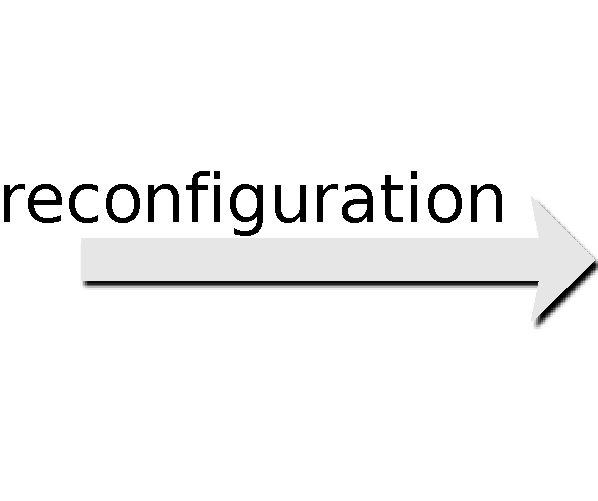
\includegraphics[width=2cm]{img/arrow_reconfiguration}
\end{minipage}
\begin{minipage}[b]{0.40\textwidth}
\begin{lstlisting}
N1: VM1 VM4
N2: VM3 VM2
?: VM5
\end{lstlisting}
\end{minipage}
\caption{A reconfiguration motivated by \cstr{root} constraints.}\label{fig: root}
\end{reconfiguration}

\begin{itemize}
\item \cstr{root(\{VM1,VM3\})}. This constraint is satisfied as none of the VMs were relocated during the reconfiguration
\item \cstr{root(\{VM4, VM5\})}. This constraint is satisfied as \cstr{VM4} is not running in the initial configuration while \cstr{VM5} is no longer running in the destination configuration. The constraint ignores then these VMs.
\item \cstr{root(\{VM2\})}. This constraint is not satisfied as \cstr{VM2} has been relocated from \cstr{N1} to \cstr{N2} during the reconfiguration process.
\end{itemize}



\fullVersion{
\subsection{Model}

This constraint is modeled using a domain restriction on the demanding slice associated to each of the running VMs.

\begin{equation*}
\begin{split}
\forall S \subseteq \mathcal{V},\ root(S) \triangleq &\\
&   \forall v_i \in V, d_i^h = c_i^h | \exists d_i^h \in \mathcal{D} , c_i^h \in \mathcal{C}
\end{split}
\end{equation*}

\subsection{Violation Detection}

\subsection{Availability}
\subsubsection{In {\btrp}} This constraint is available in {\btrp} since the version 2.0 using the name \texttt{Root}.
Using the global constraint catalog, the assignment of the d-slice placement variable is performed using a \emph{eq} constraint.

\begin{equation*}
\begin{split}
\forall S \subseteq \mathcal{V},\ root(S) \triangleq &\\
&   \forall v_i \in V, eq(d_i^h, c_i^h) | \exists d_i^h \in \mathcal{D} , c_i^h \in \mathcal{C}
\end{split}
\end{equation*}
}


\subsection{See also}

\subsubsection{Related Constraints}
\begin{itemize}
\item \cstrref{fence}: The \cstr{root} constraint can be emulated using a \cstr{fence} constraint when its user knows the current host of the specified VMs. For each VM, the list of servers given in the \cstr{fence} constraint is a singleton only composed of the current hosting server.
\end{itemize}

\printListOfInheritance{root}
\clearpage
% !TEX root =  ../main.tex
\section{Ban}
\subsection{Definition}

\subsubsection{Signature} \cstr{ban(vs : set<VM>, ns : set<server>)}

\begin{itemize}
\item \cstr{vs} : an non-empty set of VMs for a meaningful constraint. VMs not in the \st{Running} state are ignored.
\item \cstr{ns} : an non-empty set of servers for a meaningful constraint. Servers not in the \st{Online} state are ignored.
\end{itemize}

The \cstr{ban} constraint disallows each running VM in \cstr{vs} to be hosted on any of
the online servers in \cstr{ns}.

\classification{ban}{datacenter administrator}{VM placement}{Maintenance,Partitioning,VM-to-server placement}

\subsubsection{Usage}

This constraint may be use by the datacenter administrator to prepare servers for a software maintenance.
In this situation, the administrator must first be sure that the servers do not host any running VMs to prevent a
misconfiguration from altering them. Every running VM on these servers must then be relocated elsewhere
while the other VMs should not be relocated on the servers to put into maintenance.
%
A datacenter administrator may rely on a \cstr{ban} constraint to achieve that purpose. In this setting, all
the VMs in the datacenter are given in parameters in addition to the servers to put into maintenance. At the end
of the reconfiguration, no VMs will be running on the servers.  Once the maintenance operation is terminated,
the constraint may be removed to put the servers back into the hosting pool.

For partitioning reasons, some VMs may be disallowed to be running on some servers.  As an example, servers may be dedicated to run service VMs. In this setting, the client VMs must not be allowed to run on the servers dedicated to run service VMs. \cstr{Ban} constraints may then be used by the datacenter administrator for that purpose.


\subsubsection{Example}

Figure~\ref{lst: ban} depicts a sample reconfiguration between a source and a destination configuration.
In this example, the following \cstr{ban} constraints were considered:

\begin{reconfiguration}[htb]
\centering
\begin{minipage}[b]{0.40\textwidth}
\begin{lstlisting}
N1: VM1 VM2
N2: VM4 VM3
N3: 
\end{lstlisting}
\end{minipage}
\begin{minipage}[b]{2cm}
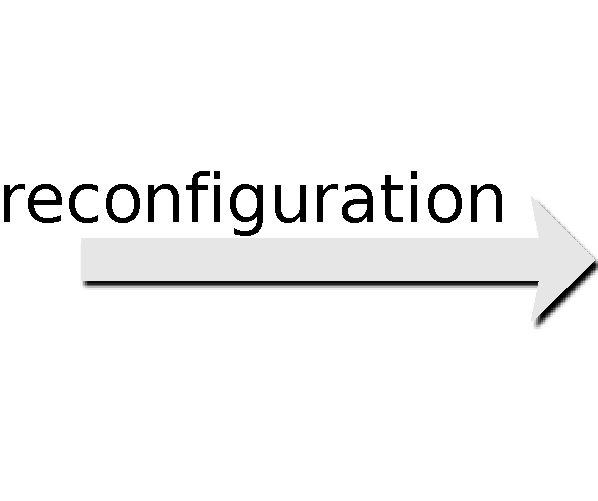
\includegraphics[width=2cm]{img/arrow_reconfiguration}
\end{minipage}
\begin{minipage}[b]{0.40\textwidth}
\begin{lstlisting}
N1: VM1
N2: (VM3)
N3: VM2 VM4
\end{lstlisting}
\end{minipage}
\caption{A reconfiguration motivated by \cstr{ban} constraints.}\label{lst: ban}
\end{reconfiguration}

\begin{itemize}
\item \cstr{ban(\{VM1, VM2, VM4\}, \{N2\})}. This constraint was not satisfied in the source configuration
as \cstr{VM4} was running on \cstr{N2}. The reconfiguration fixed this violation
by relocating \cstr{VM4} to \cstr{N3}.

\item \cstr{ban(\{VM3\}, \{N2\})}. This constraint was not satisfied in the source configuration. However it is satisfied in the destination configuration as \cstr{VM3} is no longer running.

\item \cstr{ban(\{VM1, VM2\}, \{N2\})}. This constraint was satisfied in the source configuration. It is still satisfied in the destination configuration as the relocation of \cstr{VM2} is compatible with this constraint.
\end{itemize}

\fullVersion{
\subsection{Model}

The \cstr{ban} constraint is modeled using a domain restriction on the d-slice associated to each of the running VMs.

\begin{equation*}
\begin{split}
\text{\cstr{ban(V : set<VM>, N : set<server>)}} &\triangleq\\
   & \forall v_i \in V, d_i^h \ni \{\forall j | n_j \in N\}
\end{split}
\end{equation*}

\subsection{Violation Detection}

The detection of the violating elements in \cstr{ban} consists in identifying the VMs that are hosted
on forbidden servers. The computed selection of misplaced VMs is guarantee to be minimal with regards to the scope of the constraint.

\subsection{Availability}

\subsubsection{In {\btrp}}

This constraint is available in {\btrp} using the name \texttt{ban}.
Using the Choco API, the assignment of the d-slice placement variable is pruned to remove the disallowed servers using a \emph{notMember} constraint (referred as \emph{not\_in} in the Global Constraints Catalog~\cite{gccat}).

\begin{equation*}
\begin{split}
\text{\cstr{ban(V : set<VM>, N : set<server>)}} &\triangleq\\
   & \forall v_i \in V, not\_in(d_i^h, \{\forall j | n_j \in N \})
\end{split}
\end{equation*}

\subsubsection{In VMWare}
}

\subsection{See also}

\subsubsection{Related Constraints}

\begin{itemize}
\item \cstrref{fence}: the opposite constraint of \cstr{ban}. One \cstr{ban} constraint can be emulated using a \cstr{fence} constraint by specifying to the \cstr{fence} constraint, the absolute complement of the set of servers specified in the \cstr{ban} constraint.

\item \cstrref{quarantine}. The \cstr{quarantine} constraint may also be used to prepare a software maintenance on servers when relocation is not possible. In this setting, the given servers will be ready for the maintenance once their VMs are terminated.
\end{itemize}

\emulatedWith{ban}{fence}{\cstr{ban(vs1, ns1)}}{\cstr{fence(vs1,\oline{ns1})}}
\emulatedWith{ban}{among}{\cstr{ban(vs1, ns1)}}{\cstr{among(vs1,\{\oline{ns1}\})}}
\printListOfInheritance{ban}
\clearpage
% !TEX root =  ../main.tex
\section{Fence}
\subsection{Definition}

\subsubsection{Signature} \cstr{fence(s1 : set<VM>, s2 : set<server>)}

\begin{itemize}
\item \cstr{s1} : an non-empty set of VMs for a meaningful constraint. VMs not in the \st{Running} state are ignored.
\item \cstr{s2} : an non-empty set of servers or the constraint is sure of not being satisfiable.
Servers not in the \st{Online} state are ignored.
\end{itemize}

The \cstr{fence} constraint forces each running VM in \cstr{s1} to be running on one of
the online servers in \cstr{s2}. 

\classification{fence}{datacenter administrator}{VM placement}{Partitioning,VM-to-server placement}

\subsubsection{Usage}

A \cstr{fence} constraint deserves partitioning purposes. First, it may be used by a datacenter administrator to part the infrastructure. Such a situation is typically motivated for security or administrative purposes. As an example, a datacenter may be the property of multiple organizations that have aggregated their servers. However, administrative policies may disallow to have specific VMs of one organization running on servers belonging to another organization. In this setting, \cstr{fence} constraints may be used to specify the list of allowed servers for these VMs.

Another possible usage of \cstr{fence} constraints consist in splitting the VMs when the infrastructure is designed using an aggregation of independent partitions of servers. As an example, a partition may consist of a standalone shipping container of servers or all the servers connected to a same storage space when VMs disk images are only available to these servers. In this setting, \cstr{fence} constraint allow the datacenter administrator to restrict the placement of the VMs to their assigned partition.

Finally, a \cstr{fence} constraint may be used as a backend for a resource matchmaking
system~\cite{condor-classad} for non-cumulative resources. As an example, a VM may require a particular
hypervisor, processor or GPU. \cstr{Fence} constraints may then be used to force the VMs to be running on compatible environments. The list of the compatible servers must be established before using the constraint. It has to be noticed that this use case is not suitable when the matchmaking is focusing shareable but finite resources such as memory or computing power.


\subsubsection{Example}

Figure~\ref{fig: fence} depicts a sample reconfiguration between a source and a destination configuration. In this example, the following \cstr{fence} constraints were considered.
\begin{itemize}

\item \cstr{fence(\{VM1,VM2\}, \{N1, N2\})}. This constraint was already satisfied in the source configuration as both VMs were running on \cstr{N1}. The constraint is still satisfied in the destination configuration despite \cstr{VM2} has been relocated to \cstr{N2} as this action is allowed by the constraint.

\item \cstr{fence(\{VM2, VM3\}, \{N2\})}. This constraint was not satisfied in the source configuration as \cstr{VM2} was not running on \cstr{N2}. Its relocation to \cstr{N2} during the reconfiguration fixed this violation. During the reconfiguration process, \cstr{VM3} has been stopped and is now in the \st{Waiting} state. The VM was then ignored by the constraint.
\end{itemize}

\begin{reconfiguration}
\centering
\begin{minipage}[b]{0.40\textwidth}
\begin{lstlisting}
N1: VM1 VM2
N2: VM3
N3:
?: VM4
\end{lstlisting}
\end{minipage}
\begin{minipage}[b]{2cm}
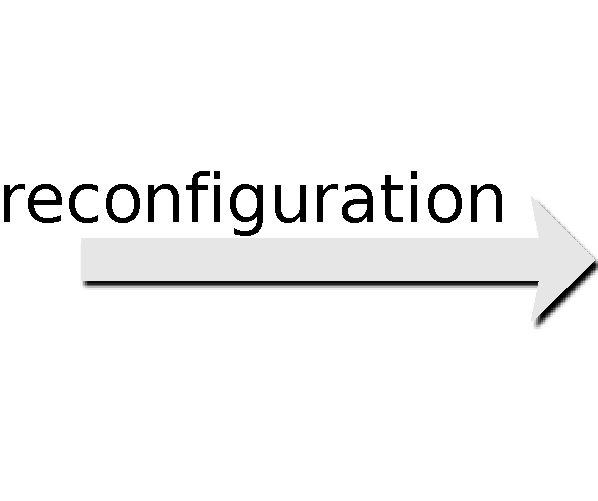
\includegraphics[width=2cm]{img/arrow_reconfiguration}
\end{minipage}
\begin{minipage}[b]{0.40\textwidth}
\begin{lstlisting}
N1: VM1 VM4
N2: VM2
N3:
?: VM3
\end{lstlisting}
\end{minipage}
\caption{A reconfiguration motivated by \cstr{fence} constraints.}\label{fig: fence}
\end{reconfiguration}

\fullVersion{
\subsection{Model}

The \cstr{fence} constraint is modeled using a domain restriction on the demanding slice associated to each of the running VMs to force each placement variable to take its value inside the values denoting
the allowed servers.

\begin{equation*}
\begin{split}
\text{\cstr{fence}}&\text{\cstr{(V : set<VM>, N : set<server>)}} \triangleq\\
 & d_i^h \in \{\forall j | n_j \in N\}, \forall v_i \in V
\end{split}
\end{equation*}

\subsection{Violation Detection}

The detection of the violating elements in \cstr{fence} consists in identifying the VMs that are not hosted
on the allowed servers. The computed selection of misplaced VMs is necessary minimal with regards to the scope of the constraint.

\subsection{Availability}

\subsubsection{In {\btrp}} This constraint is available using the name \texttt{Fence}. Using the global constraint catalog~\cite{gccat}, the domain of the d-slice placement variable is restricted to the values
denoting the allowed servers using a \emph{in} constraint. Using Choco, the domain of the variable is
directly filtered. The following denotes the model based on the global constraint catalog:

\begin{equation*}
\begin{split}
\text{\cstr{fence}}&\text{\cstr{(V : set<VM>, N : set<server>)}} \triangleq\\
	& in(d_i^h, \{\forall j | n_j \in N\}), \forall v_i \in V
\end{split}
\end{equation*}

\subsubsection{In VMWare}
}

\subsection{See also}

\subsubsection{Related Constraints}
\begin{itemize}
\item \cstrref{ban}: the opposite constraint of \cstr{fence}.
One \cstr{fence} constraint can be emulated using a \cstr{ban} constraint by specifying to the \cstr{ban} 
constraint the absolute complement of the set of servers specified in the \cstr{fence} constraint.

\item \cstrref{quarantine}: This constraint encapsulates the \cstr{fence} constraint but also disallows the VMs outside the fence to be relocated to servers inside the fence.

\item \cstrref{among}: The \cstr{among} constraint encapsulates the \cstr{fence} constraint.
The given VMs will necessarily be running on a single set of servers but multiple candidate set of servers may be passed as an argument to let the \cstr{among} constraint state about the set of servers to choose. A \cstr{fence} constraint can be emulated using one \cstr{among} constraint when only of set of servers is specified.
\end{itemize}

\emulatedWith{fence}{ban}{\cstr{fence(vs1, ns1)}}{\cstr{ban(vs1,\oline{ns1})}}
\printListOfInheritance{fence}
\clearpage
% !TEX root =  ../main.tex
\section{Quarantine}

\subsection{Definition}

\subsubsection{Signature} \cstr{quarantine(s : set<server>)}

\begin{itemize}
\item \cstr{s} : an non-empty set of servers for a meaningful constraint. Servers not in the \st{Online} state are ignored.
\end{itemize}

The \cstr{quarantine} constraint disallows any VM running on servers other than those in \cstr{s} to be relocated into a server in \cstr{s}.
%
In addition, every VM running on a server in \cstr{s} cannot be relocated to another server.
%
This constraint only restricts the placement of running VMs with regards to a previous placement.
As a result, it is not possible to state for the satisfaction of one \cstr{quarantine} constraint before a reconfiguration occurred.

\classification{quarantine}{datacenter administrator}{VM placement}{VM-to-server placement,Partitioning,Maintenance}

\subsubsection{Usage}

A \cstr{quarantine} constraint may be use by the datacenter administrator for isolation purpose.
When a server appears to be compromised, a first step to avoid to propagate
the situation is to isolate it from the datacenter (put it into \emph{quarantine}).
Using one \cstr{quarantine} constraint, the datacenter administrator is ensured that
no running VMs may enter or leave the quarantine zone.

This constraint may also be used to prepare the servers for a software maintenance operation
when it is not possible to relocate the VMs it runs.
%
To prepare a software maintenance, the datacenter administrator must be sure the server
does not host any running VMs to prevent a misconfiguration from altering them. As their relocation
is not possible in this setting, the only solution to tend to have a server ready for the maintenance
is to wait for its VMs termination while disallowing other VMs to be running on the server.
The datacenter administrator may then use a \cstr{quarantine} constraint for that purpose.


\subsubsection{Example}

Figure~\ref{fig: quarantine} depicts a sample reconfiguration between a source and a destination configuration. In this example, the following \cstr{quarantine} constraints were considered:

\begin{itemize}

\item \cstr{quarantine(\{N2\})}. This constraint is satisfied as \cstr{VM3} was not relocated while no VMs
were moved or launched to \cstr{N2}.
\item \cstr{quarantine(\{N1,N4\})}. This constraint is satisfied as \cstr{VM2} is terminated
\item \cstr{quarantine(\{N3\})}. This constraint is not satisfied as \cstr{VM5} was launched on \cstr{N3} which is in the quarantine zone.
\end{itemize}

\begin{reconfiguration}
\centering
\begin{minipage}[b]{0.40\textwidth}
\begin{lstlisting}
N1: VM1 VM2
N2: VM3
N3: VM4
(N4):
?: VM5
\end{lstlisting}
\end{minipage}
\begin{minipage}[b]{2cm}
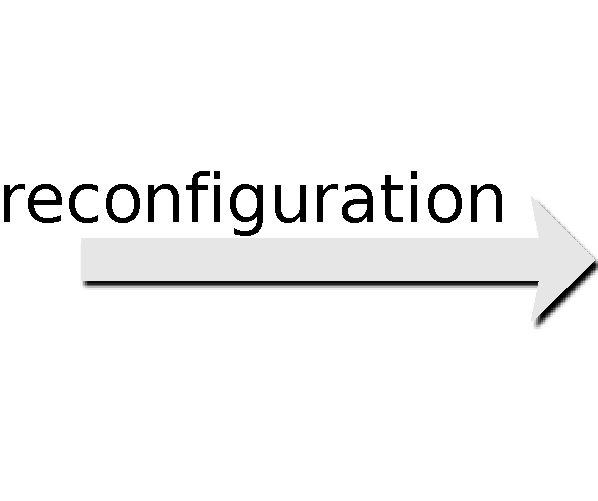
\includegraphics[width=2cm]{img/arrow_reconfiguration}
\end{minipage}
\begin{minipage}[b]{0.40\textwidth}
\begin{lstlisting}
N1: VM1
N2: VM3
N3: VM4 VM5
(N4):
?:
\end{lstlisting}
\end{minipage}
\caption{A reconfiguration motivated by \cstr{quarantine} constraints.}\label{fig: quarantine}
\end{reconfiguration}

\fullVersion{
\subsection{Model}

This constraint is modeled using domain restrictions on the demanding slice of the VMs.

\begin{equation*}
\begin{split}
\forall N \subset \mathcal{N}, \ quarantine(N) \triangleq&\\
&\forall v_i \in \mathcal{V} | v_i^h \in \bigcup_{j | n_j \in N}, d_i^h = c^h \\
&\forall v_i \in \mathcal{V} | v_i^h \ni \bigcup_{j | n_j \in N}, d_i^h \ni \bigcup_{j | n_j \in N}
\end{split}
\end{equation*}

\subsection{Violation Detection}

\subsection{Availability}
\subsubsection{In {\btrp}} 
This constraint is available in {\btrp} since the version 2.0 using the name \texttt{Quarantine}.
Using the global constraint catalog, the assignment of the d-slice placement variable in the quarantine
zone is restricted using \emph{in} constraints while VMs outside the quarantine zone are prevented to 
be relocated on the nodes in the quarantine using \emph{not\_in} constraints.

\begin{equation*}
\begin{split}
\forall N \subset \mathcal{N}, \ quarantine(N) \triangleq&\\
&\forall v_i \in \mathcal{V} | v_i^h \in \bigcup_{j | n_j \in N}, eq(d_i^h, c_i^h) \\
&\forall v_i \in \mathcal{V} | v_i^h \ni \bigcup_{j | n_j \in N}, not\_in(d_i^h, \bigcup_{j | n_j \in N})
\end{split}
\end{equation*}
}
\subsection{See also}

\subsubsection{Related Constraints}
\begin{itemize}
\item \cstrref{ban}: When it is possible to relocate the VMs, a \cstr{ban} constraint may be use to prepare servers for a software maintenance operation. In this setting, the server will be ready for the maintenance sooner as the VMs will be immediately relocated while the datacenter administrator has to wait for their termination when a \cstr{quarantine} constraint is used.

\item \cstrref{fence} $+$ \cstrref{root}. This composition of constraints
emulates a \cstr{lonely} constraint. One \cstr{fence} constraint will disallow the VMs outside the quarantine zone to enter it while one \cstr{root} constraint will prevent the relocation of the VMs running into the quarantine zone.

\item \cstrref{lonely}. A partitioning constraint to isolate VMs rather than servers.
\end{itemize}

\emulatedWith{quarantine}{fence,root}{\cstr{quarantine(s)}}{\cstr{root({\tuparrow}s), fence(\oline{{\tuparrow}s}, \oline{s})}}
\printListOfInheritance{quarantine}
\clearpage
% !TEX root =  ../main.tex
\section{Among}
\subsection{Definition}

\subsubsection{Signature} \cstr{among(vs : set<VM>, ns : set<set<server>>)}

\begin{itemize}
\item \cstr{vs} : an non-empty set of VMs for a meaningful constraint. VMs not in the \st{Running} state are ignored.
\item \cstr{ns} :  an non-empty set of set of servers or the constraint is sure of not being satisfiable.
Sets composing \cstr{ns} must be disjoint. Servers not in the \st{Online} state are ignored.
\end{itemize}

The \cstr{among} constraint forces each running VM in \cstr{vs} to be hosted on one of the set of servers in \cstr{ns}.

\classification{among}{application administrator,datacenter administrator}{VM placement}{Partitioning,VM-to-VM placement,VM-to-server placement,Performance}


\subsubsection{Usage}

The \cstr{among} constraint may be used by a datacenter administrator or
an application administrator to group closely related VMs with regards to specific criteria.
%
A datacenter network is usually designed as a fat-tree~\cite{leiserson1985fat,al2008scalable} that
provides a non-uniform network latency and bandwidth between the servers.
An application administrator having strongly communicating VMs may then require
to have its VMs hosted on servers connected to a same edge switch to improve
their communication. This  can be achieved using one \cstr{among} constraint
where each set of servers denotes the servers connected to a same edge switch.

A datacenter administrator may also rely on \cstr{among} constraints to part the datacenter
and ease its management.
%
First, the administrator reflects, using disjoint set of servers, the current physical partitioning (different geographical sites, administrative zones, shipping containers of servers~\cite{containers}, \dots) of the datacenter.
%
\cstr{Among} constraints are then use to force groups of VMs to stay inside a single physical
partition.
 

\subsubsection{Example}

Figure~\ref{lst: among} depicts a sample reconfiguration between a source and a destination configuration.
In this example, the following \cstr{among} constraints were considered:

\begin{itemize}
\item \cstr{among(\{VM1, VM2, VM3\}, \{\{N1, N2\},\{N3, N4\}\})}. This constraint was not satisfied in the
source configuration as \cstr{VM1} and \cstr{VM2} were running on the partition \cstr{\{N1, N2\}}
while \cstr{VM3} was running on the partition \cstr{\{N3, N4\}}. The reconfiguration fixed this
violation by relocating \cstr{VM3} to \cstr{N2}. \cstr{VM2} was relocated to \cstr{N2} but this action
does not contradict the constraint.

\item \cstr{among(\{VM4, VM5\}, \{\{N1\},\{N2, N3, N4\}\})}. This constraint was not satisfied in the source configuration as \cstr{VM4} and \cstr{VM5} were running on distinct partitions. This violation was fixed by
suspending \cstr{VM5}.

\item \cstr{among(\{VM6, VM7\}, \{\{N1,N2\},\{N3, N4\}\})}. This constraint was already satisfied in the source configuration as both VMs were running on the partition \cstr{\{N1,N2\}}. The constraint is still satisfied in the destination configuration as both VMs have been relocated to the partition \cstr{\{N3,N4\}}.

\end{itemize}

\begin{reconfiguration}
\centering
\begin{minipage}[b]{0.40\textwidth}
\begin{lstlisting}
N1: VM1 VM2 VM6 VM7
N2: VM5
N3: VM3
N4: VM4 
\end{lstlisting}
\end{minipage}
\begin{minipage}[b]{2cm}
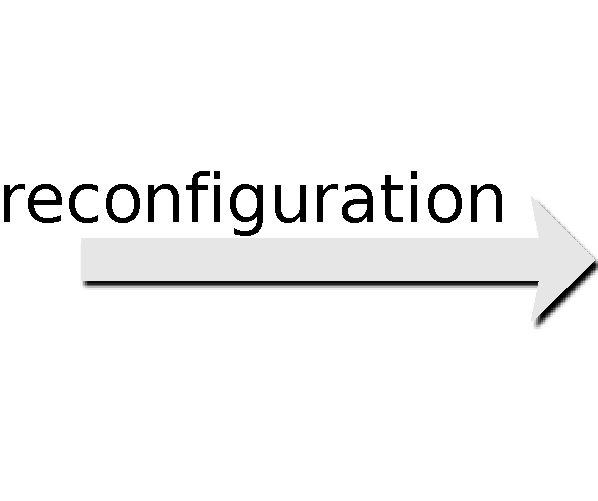
\includegraphics[width=2cm]{img/arrow_reconfiguration}
\end{minipage}
\begin{minipage}[b]{0.40\textwidth}
\begin{lstlisting}
N1: VM1 
N2: VM2 VM3 (VM5)
N3: VM6
N4: VM4 VM7
\end{lstlisting}
\end{minipage}
\caption{A reconfiguration motivated by \cstr{among} constraints.}\label{lst: among}
\end{reconfiguration}


\fullVersion{
\subsection{Model}

To implement \cstr{among}, each of the servers group is identified by a constant.
A variable $G$ is then created to indicate the group hosting the VMs. 
$G$ is linked to each of the d-slice placement variables to indicate
that if a d-slice of one of the given VM is hosted on a server, then all the VMs are
hosted on the set of servers to which this server belongs to. The equation~\eqref{eq: rp among}
depicts this model.
\todo{incorrect}
\begin{equation*}
\begin{split}
\text{\cstr{among}} & \text{\cstr{(V : set<VM>, S : set< set<server> >)}} \triangleq\\
& G \in <0.. card(S) - 1> \\
& \forall v_i \in V, d_i^{host} = j \imply 
G = j \leftrightarrow d_i^{host} \in S_j
\end{split}\label{eq: rp among}
\end{equation*}

\subsection{Availability}

\subsubsection{In {\btrp}}

The constraint \cstr{among}�is available in {\btrp}�since the version 2.1.
Each of the server groups is identified by a constant, and a variable is created to
indicate the selected group.  This variable is linked to each of the
d-slice placement variables using the \emph{nth} constraint, indicating
that if a d-slice of one of the given VM is hosted on a server, then all
the given VMs are hosted on the set of servers to which this server
belongs.

\subsection{Violation detection}

The \cstr{among} constraint restricts a VM placement relatively to the others.
If two VMs are assigned to different group of servers, it is then not possible
to detect which group is the \emph{right one}. To avoid to underestimate
the misplaced VMs, a safe approach consists in selecting every VMs
when they are placed on different group of servers. 
}


\subsection{See also}

\subsubsection{Related Constraints}
\begin{itemize}
\item \cstrref{fence}: The \cstr{fence} constraint is a specialization of the \cstr{among} constraint: only one set of servers is possible to restrict the VMs placement. A \cstr{among} constraint is then equivalent to a \cstr{fence} constraint when there is only one possible set of servers to host the VMs. This  occurs when only one set of servers is specified, when other sets are offline, or when one of the given VMs is ensured to be hosted on a known server as the other VMs will necessarily be hosted on the set of servers the known server belong to.

\end{itemize}
\emulatedWith{among}{splitAmong}{\cstr{among(vs1, ns1)}}{\cstr{splitAmong(\{vs1\},ns1)}}
\printListOfInheritance{among}
\clearpage
% !TEX root =  ../main.tex
\section{Lonely}

\subsection{Definition}

\subsubsection{Signature} \cstr{lonely(s : set<VM>)}

\begin{itemize}
\item \cstr{s} : an non-empty set of VMs for a meaningful constraint. VMs not in the \st{Running} state are ignored.
\end{itemize}

The \cstr{lonely} constraint forces all the running VMs in \cstr{s} to be running on dedicated servers.
Each of the used servers can still host multiple VMs but they have to be in \cstr{s}.

\classification{lonely}{application administrator}{VM placement}{VM-to-VM placement,Partitioning}

\subsubsection{Usage}

The \cstr{lonely} constraint deserves isolation purposes. Hypervisors are supposed
to provide a strong isolation between the VMs. However various attacks, such as those based on 
VM escaping~\cite{wojtczuk},
allow to break this isolation to provide from a malicious VM, a non-legitimate access to the hypervisor or the other VMs.
An application administrator may then want to have to prevent this situation by requiring to have its VMs hosted on servers that do not host unknown, potentially malicious VMs. A \cstr{lonely} constraint can then be used to indicate the VMs that must be running on dedicated servers.

\subsubsection{Example}

Figure~\ref{fig: lonely} depicts a sample reconfiguration between a source and a destination configuration. In this example, the following \cstr{lonely} constraints were considered:

\begin{reconfiguration}
\centering
\begin{minipage}[b]{0.40\textwidth}
\begin{lstlisting}
N1: VM1 VM2
N2: VM3
N3: VM4
N4: VM6
N5: VM5
\end{lstlisting}
\end{minipage}
\begin{minipage}[b]{2cm}
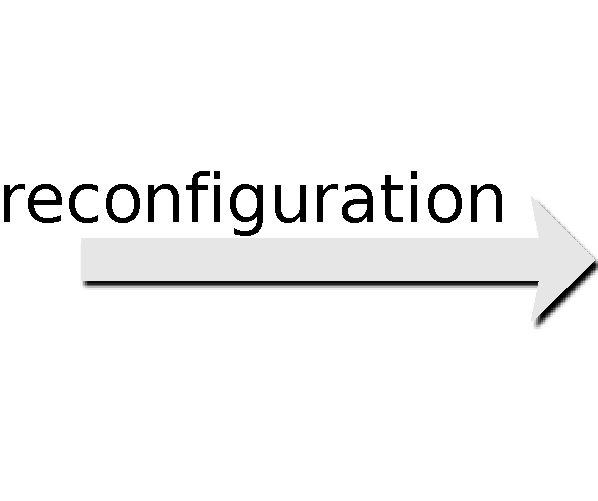
\includegraphics[width=2cm]{img/arrow_reconfiguration}
\end{minipage}
\begin{minipage}[b]{0.40\textwidth}
\begin{lstlisting}
N1: VM1
N2: VM3
N3: VM2 VM4
N4: VM6 VM5
N5:
\end{lstlisting}
\end{minipage}
\caption{A reconfiguration motivated by \cstr{lonely} constraints.}\label{fig: lonely}
\end{reconfiguration}

\begin{itemize}

\item \cstr{lonely(\{VM1,VM3\})}. This constraint was not satisfied in the source configuration as \cstr{VM2}
was colocated with \cstr{VM1} despite \cstr{VM2} does not belong to the VMs given as parameter.
This violation was fixed by relocating \cstr{VM2} to \cstr{N3}.

\item \cstr{lonely(\{VM2, VM4\})}. This constraint was not satisfied in the source configuration. It was fixed by
colocating \cstr{VM2} with \cstr{VM4} on \cstr{N3}.

\item \cstr{lonely(\{VM5, VM6\})}. This constraint was satisfied in the source configuration.
The constraint is still satisfied in the destination configuration despite the relocation of \cstr{VM5} to
\cstr{N4} which is allowed by the constraint.
\end{itemize}


\fullVersion{
\subsection{Model}

This constraint is modeled using a restriction on the demanding slice associated to each of the running VMs.

\begin{equation*}
\begin{split}
\forall V \subseteq \mathcal{V}, \ lonely(V) \triangleq&\\
   & \forall v_i,v_j \in V, d_i^h =  d_j^h
\end{split}
\end{equation*}

\subsection{Violation Detection}

The detection of the violating elements in \cstr{lonely} consists in computing every VMs that are not
in the given set of VMs, but running on servers hosting the given VMs.


\subsection{Availability}

\subsubsection{In {\btrp}}

This constraint is available in {\btrp} since the version 2.1 using the name \texttt{Lonely}. 
Two groups of placement variables are created. One containing the placement variables of the given VMs, the other containing the other VMs running on the servers. One \emph{disjoint} ensures then
no variables in different groups, are instantiated to the same value.

\begin{equation*}
\begin{split}
\forall V \subseteq \mathcal{V}, \ lonely(V) \triangleq&\\
   & \forall v_i,v_j \in V, eq(d_i^h, d_j^h)
\end{split}
\end{equation*}

\subsubsection{In Amazon EC2}

The constraint is available on Amazon EC2 under the terms of \emph{dedicated instances}~\cite{amazon-lonely}.
}

\subsection{See also}

%\subsubsection{Context relative constraints}

%\begin{itemize}
%\item \cstrref{split}: The \cstr{split} constraint is a generalization of the \cstr{lonely} constraint. It states that the two set of VMs, given as arguments,  must not share servers. A \cstr{lonely} constraint can then be emulated using a \cstr{split} constraint when the second set of VMs is the absolution complement of the first one.
%\end{itemize}

%\subsubsection{Emulating the \cstr{lonely} constraint}
\emulatedWith{lonely}{split}{\cstr{lonely(vs1)}}{\cstr{split(\{vs1,\oline{vs1}\})}}
\printListOfInheritance{lonely}
%\begin{itemize}
%\item 
%\end{itemize}
%
%\subsubsection{Available specializations of the \cstr{lonely} constraint}





\clearpage
% !TEX root =  ../main.tex
\section{Split}

\subsection{Definition}

\subsubsection{Signature} \cstr{split(vs: set<set<VM>>)}

\begin{itemize}
\item \cstr{vs} : a non-empty set of set of VMs for a meaningful constraint. VMs not in the \st{Running} state are ignored. Sets inside \cstr{vs} must be disjoint.
\item \cstr{s2} : an non-empty set of VMs for a meaningful constraint, that is distinct from \cstr{s1}. VMs not in the \st{Running} state are ignored.
\end{itemize}

The \cstr{split} constraint forces the given sets of VMs in \cstr{vs} to not share hosting servers.
Each of the used servers can still host multiple VMs but they have to be in the same set.

\classification{split}{application administrator}{VM placement}{VM-to-VM placement,Partitioning,Fault tolerance}

\subsubsection{Usage}

The \cstr{split} constraint deserves isolation requirements. Hypervisors are supposed
to provide a strong isolation between the VMs.  However, various attacks such as those based on 
VM escaping~\cite{wojtczuk}, allow to break this isolation to provide from a malicious VM, a non-legitimate access to the hypervisor or the other VMs.
An application administrator may then want to have its VMs hosted on servers that do not
host potentially malicious VMs. A \cstr{split} constraint may then be used to indicate the VMs that must be running on servers other than the supposed malicious ones.

The \cstr{split} constraint deserves also fault tolerance requirements. For high-availability purposes,
replicated applications are supposed to be running on distinct servers. In this setting, an application
administrator may use one \cstr{split} constraint to ensure all the VMs of the application do not
share any server with the replicated VMs.

\subsubsection{Example}

Figure~\ref{fig: split} depicts a sample reconfiguration between a source and a destination configuration. In this example, the following \cstr{split} constraints were considered:

\begin{reconfiguration}
\centering
\begin{minipage}[b]{0.40\textwidth}
\begin{lstlisting}
N1: VM1 VM2
N2: VM3
N3: VM4 VM5
N4: VM6
N5: VM7 VM8
\end{lstlisting}
\end{minipage}
\begin{minipage}[b]{2cm}
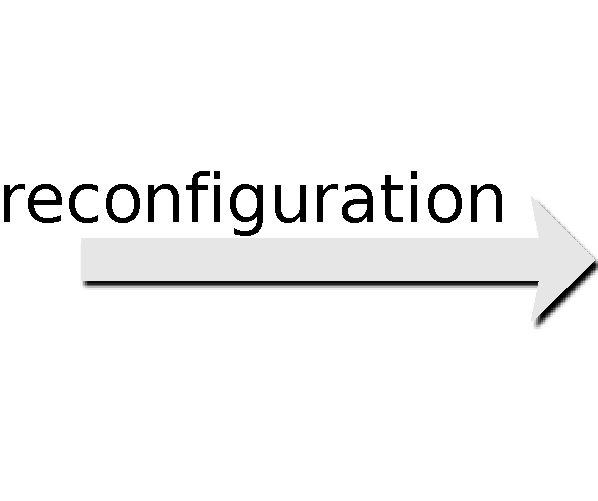
\includegraphics[width=2cm]{img/arrow_reconfiguration}
\end{minipage}
\begin{minipage}[b]{0.40\textwidth}
\begin{lstlisting}
N1: VM1
N2: VM3
N3: VM2 VM4 VM5
N4: VM7 (VM6)
N5: VM8
\end{lstlisting}
\end{minipage}
\caption{A reconfiguration motivated by \cstr{split} constraints.}\label{fig: split}
\end{reconfiguration}


\begin{itemize}

\item \cstr{split(\{\{VM1,VM3\},\{VM2, VM4\}\})}. This constraint was not satisfied in the source configuration as
\cstr{VM2} and \cstr{VM1} were colocated despite they belong to different sets. This violation was fixed
by relocating \cstr{VM2} to \cstr{N3}.

\item \cstr{split(\{\{VM5,VM6\},\{VM7, VM8\}\})}. This constraint was satisfied in the sour\-ce configuration as no set of VMs share hosts. The constraint is still satisfied in the destination configuration: despite \cstr{VM7} and \cstr{VM6} are on the same server, \cstr{VM6} is not in the \st{Running} state, so it is ignored by the constraint.

\end{itemize}

\fullVersion{
\subsection{Model}

The \cstr{split} is modeled by restricting the placement of each d-slice placement variable for
one group to not take any value that is in the other group

\begin{equation*}
\begin{split}
\forall V_1,V_2 \subseteq \mathcal{V} & split(V_1,V_2) \triangleq \\
& \forall v_i \in V_1, v_j \in V_2, d_i^{host} \neq d_j^{host}
\end{split}
\end{equation*}

\subsection{Violation Detection}

The detection of the violating elements in \cstr{split} consists
in computing the sets of used servers for each group of VMs.
The intersection of the two set of servers reveals the misplaced VMs.
This set of VMs is not minimal as only the VMs from one group will have to leave
on each of these server.

\subsection{Availability}

\subsubsection{In {\btrp}}

This constraint in available in {\btrp} since version 2.1.

\begin{equation*}
\begin{split}
\forall V_1,V_2 \subseteq \mathcal{V} & split(V_1,V_2) \triangleq \\
& disjoint(\{d_i, \forall v_i \in V_1\}, \{d_j, \forall v_j \in V_2\})
\end{split}
\end{equation*}
}

\subsection{See also}

\subsubsection{Related Constraints}
\begin{itemize}
\item \cstrref{spread}, \cstrref{lazySpread}: These constraints
disallow the colocation between VMs rather than groups of VMs.
A \cstr{split} constraint is equivalent to a \cstr{lazySpread} constraint when the \cstr{split} constraint is made up with two sets of one VM each.
\item \cstrref{splitAmong}: This constraint forces several set of VMs to be hosted on distinct groups of servers among those explicitly allowed.
\item \cstrref{lonely}. The \cstr{lonely} constraint is a specialization of the \cstr{split} constraint that isolate a set of VMs from all the others. It can then be emulated using a \cstr{split} constraint when the second set of VMs is the absolution complement of the first one.
\end{itemize}

\printListOfInheritance{split}
\clearpage
% !TEX root =  ../main.tex
\section{SplitAmong}

\subsection{Definition}

\subsubsection{Signature} \cstr{splitAmong(vs : set<set<VM>>, ns : set<set<server>>)}

\begin{itemize}
\item \cstr{vs} : a non-empty set of set of VMs for a meaningful constraint. VMs not in the \st{Running} state are ignored. Sets inside \cstr{vs} must be disjoint.
\item \cstr{ns} : a set of set of servers that is composed of more sets than \cstr{vs} or the constraint is sure of not being satisfiable.
Sets composing \cstr{ns} must be disjoint. Servers not in the \st{Online} state are ignored.
\end{itemize}

The \cstr{splitAmong} constraint forces the sets of VMs inside \cstr{vs}
to be hosted on distinct set of servers in \cstr{ns}. VMs inside a same set may still be collocated.

\classification{splitAmong}{application administrator}{VM placement}{VM-to-VM placement,Partitioning,Fault tolerance}

\subsubsection{Usage}

The \cstr{splitAmong} constraint deserves isolation requirements. One solution to ensure disaster recovery for an application is to replicate it. When the master application fail, the replica is activated transparently to neglect the failure effect. In practice, the replication is a mechanism provided at the hypervisor level~\cite{remus,vmwareFT}. The replicas are then placed to a distant server to make the application survive
to a datacenter failure. One application administrator may obtain this fault tolerance using one \cstr{splitAmong} constraint. The sets of VMs given as parameters are the master then the slave VMs while the
set of servers are the servers composing each datacenter.

\subsubsection{Example}

Figure~\ref{fig: splitAmong} depicts a sample reconfiguration between a source and a destination configuration. In this example, the following \cstr{splitAmong} constraints were considered:

\begin{reconfiguration}
\centering
\begin{minipage}[b]{0.40\textwidth}
\begin{lstlisting}
N1: VM1 VM2
N2: VM3
N3: VM4 VM5
N4: VM6
N5: VM7 VM8
\end{lstlisting}
\end{minipage}
\begin{minipage}[b]{2cm}
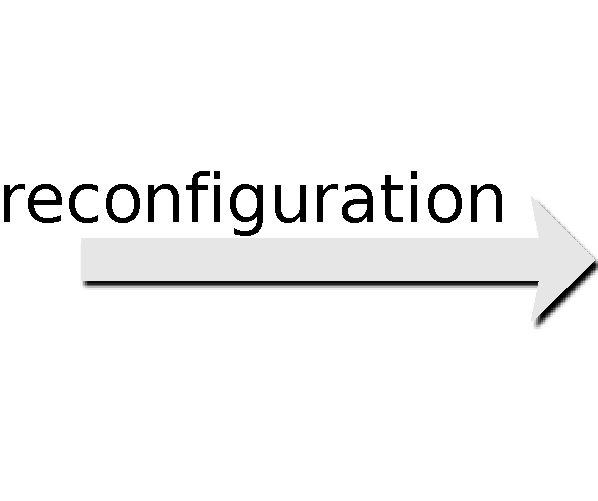
\includegraphics[width=2cm]{img/arrow_reconfiguration}
\end{minipage}
\begin{minipage}[b]{0.40\textwidth}
\begin{lstlisting}
N1: VM1
N2: VM3
N3: VM2 VM4 VM5
N4: VM7 VM6
N5: (VM8)
\end{lstlisting}
\end{minipage}
\caption{A reconfiguration motivated by \cstr{splitAmong} constraints.}\label{fig: splitAmong}
\end{reconfiguration}


\begin{itemize}

\item \cstr{splitAmong(\{\{VM1,VM3\},\{VM2,VM4\}\},\{\{N1,N2\},\{N3,N4\}\})}. This constraint was not satisfied in the source configuration as \cstr{VM2} and \cstr{VM1} were both running inside the set of servers \cstr{\{N1,N2\}} despite they belong to different sets of VMs. In addition, the set of VMs \cstr{\{VM2,VM4\}} was spread among the two set of servers while it should be running on only one. These violations were fixed by relocating \cstr{VM2} to \cstr{N4} to let the first set of VMs running on the first set of servers and the second set of VMs running on the second set of servers.

\item \cstr{splitAmong(\{\{VM1,VM3\},\{VM5,VM6,VM7, VM8\}\},\{\{N1,N2\},\{N3,N4\}\})}. This constraint was not satisfied in the source configuration as \cstr{VM7} and \cstr{VM8} were running on \cstr{N5}, that does not belong to any of the allowed sets.  This violation was fixed by relocating \cstr{VM7} to \cstr{N4} and by suspending \cstr{VM8} which is now ignored by the constraint.

\item \cstr{splitAmong(\{\{VM1,VM2,VM3\},\{VM7,VM8\}\},\{\{N1,N2,N3\},\{N4,N5\}\})}.This constraint was satisfied in the source configuration as the sets of VMs share do not share a group of servers. The constraint is still satisfied in the destination configuration despite the relocation of \cstr{VM2} and \cstr{VM7} to \cstr{N3} and \cstr{N4} respectively which let them running inside their dedicated group of servers.

\end{itemize}

%Availability: FT VMWare and EC2
\subsection{See also}

\subsubsection{Related Constraints}
\begin{itemize}
\item \cstrref{split}: This constraint disallows two set of VMs to share servers.
\item \cstrref{spread}, \cstrref{lazySpread}: These constraints disallow the colocation between VMs rather than groups of VMs.
\item \cstrref{fence}: \cstr{splitAmong} is equivalent to a \cstr{fence} constraint when only one set of VMs and one set of servers are given as arguments.

\end{itemize}

\printListOfInheritance{splitAmong}
\clearpage
% !TEX root =  ../main.tex
\section{Gather}
\subsection{Definition}

\subsubsection{Signature} \cstr{gather(s : set<VM>)}

\begin{itemize}
\item \cstr{s} : a set of at least 2 VMs for a meaningful constraint. VMs not in the \st{Running} state are ignored.
\end{itemize}

The \cstr{gather} constraint forces all the running VMs in the set \cstr{s} to be hosted on the same server.

\classification{gather}{application administrator}{VM placement}{Performance,VM-to-VM placement}

\subsubsection{Usage}

The \cstr{gather} constraint may first be used by an application administrator to force the colocation of
 strongly communicating VMs.
Using one \cstr{gather} constraint, the VMs will be running on a same server and the virtual network between them will be embedded into the internal network provided by the hypervisor instead of the physical network, leading to better network performance.

The \cstr{gather} constraint may also be used by an application administrator to force the colocation
of VMs that have to share a component such as a filesystem. Without any guarantee of colocation, it is a necessary to rely on a distributed filesystem or a file server which provide less performance than a raw and direct access to the data. Using the colocation guarantee provided by a \cstr{gather} constraint, the filesystem
may be placed directly on the hosting server to achieve better performance. In this context, it is also often
desirable to use one \hyperref[cstr: root]{\cstr{root}} constraint to prevent from VMs relocation.

It has however to be noticed that these usages ask explicitly for the VMs colocation. It is then not allowed to host the VMs on several servers when the colocation is not possible. The application administrator should then  not over-estimate his needs to prevent him from having its VMs not running at all.

\subsubsection{Example}

Figure~\ref{fig: gather} depicts a sample reconfiguration between a source and a destination configuration. In this example, the following \cstr{gather} constraints were considered:

\begin{itemize}

\item \cstr{gather(\{VM1, VM4\})}. This constraint was satisfied in the source configuration as only \cstr{VM1}
was running, so considered in the constraint. The constraint is also satisfied in the destination configuration:
during the reconfiguration, \cstr{VM4} was set in the \st{Running} state and deployed on \cstr{N1} according to
the constraint requirement.

\item \cstr{gather(\{VM2, VM5\})}. This constraint was not satisfied in the source configuration as \cstr{VM4} and \cstr{VM5} were running on different servers. The reconfiguration fixed this violation by relocating \cstr{VM2} to \cstr{N3} which is also hosting \cstr{VM5}.

\item \cstr{gather(\{VM3, VM6\})}. This constraint was satisfied in the source configuration as both VMs were running on \cstr{N2}. Despite both VMs were relocated during the reconfiguration process, the constraint is still satisfied in the destination configuration as both VMs are running on \cstr{N4} and the end of reconfiguration.
\end{itemize}

\begin{reconfiguration}
\centering
\begin{minipage}[b]{0.40\textwidth}
\begin{lstlisting}
N1: VM1 VM2
N2: VM3 VM6
N3: VM5
N4: 
? : VM4
\end{lstlisting}
\end{minipage}
\begin{minipage}[b]{2cm}
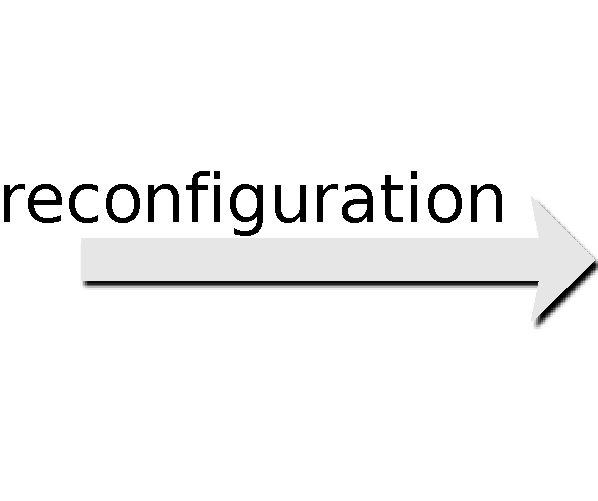
\includegraphics[width=2cm]{img/arrow_reconfiguration}
\end{minipage}
\begin{minipage}[b]{0.40\textwidth}
\begin{lstlisting}
N1: VM1 VM4
N2:
N3: VM5 VM2
N4: VM3 VM6
? :
\end{lstlisting}
\end{minipage}
\caption{A reconfiguration motivated by \cstr{gather} constraints.}\label{fig: gather}
\end{reconfiguration}

\fullVersion{
\subsection{Model}

The \cstr{gather} is modeled by forcing the d-slice placement variable associated to each running VM to be equal. In terms of RP variable, the constraint is modeled as follow:

\begin{equation*}
\begin{split}
\text{\cstr{gather(V : set<VM>)}}&\triangleq\\
&\forall v_i, v_j \in V, d_i^h = d_j^h
\end{split}
\end{equation*}

\subsection{Violation Detection}

The detection of the violating elements in \cstr{gather} consists in computing all the current hosting servers for the given running VMs. If there is only one server, then there is no misplaced VMs. Otherwise, there must be misplaced VMs. There is no safe solutions to detect the exact VMs that are misplaced within the scope of a \cstr{gather} constraint as each of the hosting server may be the \emph{right one}. It is however possible to count the minimal number of misplaced VMs. In practice, it is equals to the minimal number of involved VMs hosted on one of the servers.

\subsection{Availability}

\subsubsection{In {\btrp}}

This constraint is available in {\btrp} using the name \texttt{Gather}. Using the global constraint catalog~\cite{gccat}, the assignment of all the d-slice placement variables is ensure to be the same using \emph{eq} constraints. In practice, the \cstr{gather} constraint is modeled as follow:

\begin{equation*}
\begin{split}
\text{\cstr{gather(V : set<VM>)}}&\triangleq\\
   & \forall v_i,v_j \in V, eq(d_i^h, d_j^h)
\end{split}
\end{equation*}

\subsubsection{In VMWare}

Affinity rules between VMs allows to reproduce the \cstr{gather} constraint.
}
\subsection{See also}

\subsubsection{Related Constraints}
\begin{itemize}
\item \cstrref{spread}, \cstrref{lazySpread}: the opposite constraints of \cstr{gather} that force the VMs to be hosted on distinct servers.
\end{itemize}

\emulatedWith{gather}{among}{\cstr{gather(s)}}{\cstr{among(s,\allNodes/|\allNodes|)}}
\printListOfInheritance{gather}
\clearpage
% !TEX root =  ../main.tex
\section{Spread}

\subsection{Definition}

\subsubsection{Signature} \cstr{spread(s : set<VM>)}

\begin{itemize}
\item \cstr{s} : a set of at least 2 VMs for a meaningful constraint. VMs not in the \st{Running} state are ignored.
\end{itemize}

The \cstr{spread} constraint forces all the running VMs in \cstr{s} to be hosted
on distinct servers at any time, even during the reconfiguration process.

\classification{spread}{application administrator}{VM placement,Actions schedule}{Fault tolerance,VM-to-VM placement,Partitioning}

\subsubsection{Usage}

The \cstr{spread} constraint may be used by an application administrator to provide to a replicated service,
fault tolerance to hardware failures. By hosting each replicas on a distinct server, the service will  be
available while at least one server is still online. To achieve this purpose, one \cstr{spread} constraint can
be used with the replicas provided as arguments.


\subsubsection{Example}

Figure~\ref{fig: spread} depicts a sample reconfiguration between a source and a destination
configuration. In this example, the following \cstr{spread} constraints were considered:

\begin{reconfiguration}
\centering
\begin{minipage}[b]{0.40\textwidth}
\begin{lstlisting}
N1: VM1 VM2
N2: VM3 VM4 VM5
N3: VM6
\end{lstlisting}
\end{minipage}
\begin{minipage}[b]{2cm}
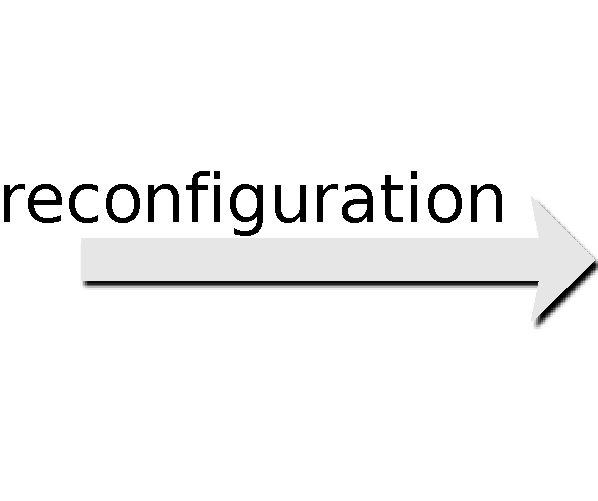
\includegraphics[width=2cm]{img/arrow_reconfiguration}
\end{minipage}
\begin{minipage}[b]{0.40\textwidth}
\begin{lstlisting}
N1: VM1 VM6
N2: VM3 (VM4)
N3: VM2 VM5
\end{lstlisting}
\end{minipage}
\caption{A reconfiguration motivated by \cstr{spread} constraints.}\label{fig: spread}
\end{reconfiguration}

\begin{itemize}

\item \cstr{spread(\{VM1,VM2\})}. This constraint was not satisfied in the source configuration as both VMs were colocated.
%
The reconfiguration fixed this violation by relocating \cstr{VM2} to \cstr{N3}.

\item \cstr{spread(\{VM3, VM4\})}. This constraint was not satisfied in the source configuration.
Putting \cstr{VM4} in the \st{Suspended} state fixed this violation without having to perform a relocation.

\item \cstr{spread(\{VM5, VM6\}}). This constraint was satisfied in the source configuration. However, let consider
\cstr{VM5} must be running on \cstr{N3}, which was already hosting \cstr{VM6}. In this setting, \cstr{VM6}
has been relocated to \cstr{N1} to disallow the colocation. Furthermore, to prevent from a temporary colocation on \cstr{N3}, it was a necessary to relocate \cstr{VM6} before \cstr{VM5}. Figure~\ref{fig: spread plan} depicts the associated event-based reconfiguration plan.
\end{itemize}


\begin{reconfPlan}[htb]
\centering
\begin{tabular}{ll}
\O & $\rightarrow$ stop(VM4) \& relocate(VM5)\\
!relocate(VM5)\ & $\rightarrow$ relocate(VM6)\\
!relocate(VM6)\ & $\rightarrow$ relocate(VM2)
\end{tabular}
\caption{Event-based reconfiguration plan associated to the reconfiguration depicted in Figure~\ref{fig: spread}.}\label{fig: spread plan}
\end{reconfPlan}

\fullVersion{
\subsection{Model}

The \cstr{spread} constraint is modeled using negations between the d-slice placement variables of the running VMs to ensure all the running VMs will be hosted on distinct servers by the end of the reconfiguration process.
To prevent from a temporary overlap during the reconfiguration process, precedence relations between the slices are established. When a d-slice associated to a VM has to be hosted on a server that is currently hosting another (but necessarily leaving) involved VM, then the relocation is delayed until the VM has leaved the server.

\begin{equation*}
\begin{split}
\text{\cstr{spread}}&\text{\cstr{(V : set<VM>)}} \triangleq\\
   & \forall v_i,v_j \in V,\\
   & d_i^h \neq d_j^h \wedge\\
   & d_i^{h} = c_j^{h} \Rightarrow d_i^{st} \geq c_j^{ed}
\end{split}
\end{equation*}

\subsection{Availability}

\subsubsection{In {\btrp}} 
This constraint is available in {\btrp} using the name \texttt{Spread}.
Using the global constraint catalog, the assigned for each of the d-slice placement variable is
ensured to be unique  using one \emph{allDifferent}~\cite{allDiff} global constraint.
The non-overlapping of VMs during the reconfiguration process is expressed by establishing an implication between constraints. \emph{Implies} constraints are used to indicate that when
the placement variable of a d-slice equals the placement of the
c-slice of any other involved
VMs  then the arrival time of the d-slice must be greater than or equal to the departure time of the
c-slice.


\begin{equation*}
\begin{split}
\text{\cstr{spread}}&\text{\cstr{(V : set<VM>)}} \triangleq\\
   & \text{\em allDifferent}(\{\forall d_i^h | v_i \in V\}) \\
   & implies(eq(d_i^h, c_i^h), geq(d_i^{st}, c_j^{ed})), \forall v_i, v_j \in V
\end{split}
\end{equation*}

\subsection{Violation Detection}

The detection of the violating elements in \cstr{spread} consists in identifying running VMs that are hosted on a same server. When a server hosts multiple VMs that are involved in a same \cstr{spread} constraint, it is ensured that at least one VM is misplaced. Such a violation detection is however not guarantee to be optimal as it is not possible to know exactly which of the colocated VMs are supposed to be hosted elsewhere. An approximation consists then to select all the colocated VMs.
}

\subsection{See also}

\subsubsection{Related Constraints}
\begin{itemize}
\item \cstrref{gather}: the opposite constraint of \cstr{spread}.
\item \cstrref{lazySpread}: a constraint similar to \cstr{spread} that does not guarantee the non-overlapping of the VMs during the reconfiguration process.
\item \cstrref{split}: a constraint to ensure two sets of VMs do not share servers.

\end{itemize}

\printListOfInheritance{spread}
\clearpage
% !TEX root =  ../main.tex
\section{LazySpread}
\subsection{Definition}

\subsubsection{Signature} \cstr{lazySpread(s : set<VM>)}

\begin{itemize}
\item \cstr{s} : a set of at least 2 VMs for a meaningful constraint. VMs not in the \st{Running} state are ignored.
\end{itemize}

The \cstr{lazySpread} constraint forces all the running VMs in \cstr{s} to be hosted on distinct servers at the end of a reconfiguration process.

\classification{lazySpread}{application administrator}{VM placement}{VM-to-VM placement,Fault tolerance,Partitioning}

\subsubsection{Usage}

The \cstr{lazySpread} constraint may be used by an application administrator to provide to a replicated service, fault tolerance to hardware failures. By hosting each replicas on a distinct server, the service will  be
available while at least one server is still online. To achieve this purpose, one \cstr{lazySpread} constraint can
be used with the replicas provided as arguments.

\subsubsection{Example}

Figure~\ref{fig: lazySpread} depicts a sample reconfiguration between a source and a destination
configuration. In this example, the following \cstr{lazySpread} constraints were considered:


\begin{reconfiguration}
\centering
\begin{minipage}[b]{0.40\textwidth}
\begin{lstlisting}
N1: VM1 VM2
N2: VM4
N3: VM3
\end{lstlisting}
\end{minipage}
\begin{minipage}[b]{2cm}
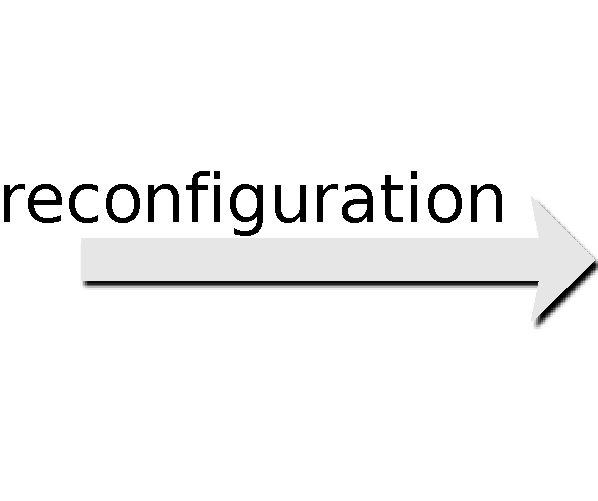
\includegraphics[width=2cm]{img/arrow_reconfiguration}
\end{minipage}
\begin{minipage}[b]{0.40\textwidth}
\begin{lstlisting}
N1: VM1
N2: (VM4) VM3
N3: VM2
\end{lstlisting}
\end{minipage}
\caption{A reconfiguration motivated by \cstr{lazySpread} constraints.}\label{fig: lazySpread}
\end{reconfiguration}

\begin{itemize}

\item \cstr{lazySpread(\{VM1, VM3, VM4\})}. This constraint was satisfied in the sour\-ce configuration as each VM were running on distinct servers. The constraint is still satisfied in the destination configuration despite \cstr{VM3} and \cstr{VM4} are colocated as \cstr{VM4} has been suspended.

\item \cstr{lazySpread(\{VM1,VM2\})}. This constraint was not satisfied in the source configuration as both VMs where running on \cstr{N1}. The relocation of \cstr{VM2} to \cstr{N3} fixed this violation.

\item \cstr{lazySpread(\{VM2, VM3\})}. This constraint was satisfied in the source configuration as both VMs were running on distinct servers. The constraint is still satisfied in the destination configuration despite the relocation of \cstr{VM2} to \cstr{N3} that was running \cstr{VM3} initially as \cstr{VM3} has been relocated elsewhere to let both VMs be running on distinct servers at the end of the reconfiguration process.
\end{itemize}


\fullVersion{
\subsection{Model}

This constraint is modeled using a negations between the d-slice placement variables of the running VMs.

\begin{equation*}
\begin{split}
\forall V \subseteq \mathcal{V}, \ lazySpread(V) \triangleq&\\
   & \forall v_i,v_j \in V, d_i^h \neq d_j^h
\end{split}
\end{equation*}

\subsection{Violation Detection}

The detection of the violating elements in \cstr{lazySpread} consists in identifying VMs that are hosted
on a same server. When a server hosts multiple VMs that are involved in the \cstr{lazySpread}
constraints, it is ensured that at least one VM is misplaced. Such a violation detection is however not guarantee to be optimal as it is not possible to know exactly which of the colocated VMs are supposed to be hosted elsewhere.

\subsection{Availability}
\subsubsection{In {\btrp}} 
This constraint is available in {\btrp} since the version 2.0 using the name \texttt{LazySpread}.
Using the global constraint catalog, the assigned for each of the d-slice placement variable is
ensured to be unique  using one \emph{allDifferent}~\cite{allDiff} global constraint.

\begin{equation*}
\begin{split}
\forall V \subseteq \mathcal{V}, \ lazySpread(V) \triangleq&\\
   & \text{\em allDifferent}(\forall d_i^h | v_i \in V)
\end{split}
\end{equation*}

\subsubsection{In VMWare DRS} 

The \emph{VM to VM} affinity rule may disallow a set of VMs to share servers.
}

\subsection{See also}

\subsubsection{Related Constraints}
\begin{itemize}
\item \cstrref{gather}: the opposite constraint of \cstr{spread}
\item \cstrref{spread}: a constraint similar to \cstr{lazySpread}
but which also guarantee that the VMs will never overlap on a same server, even during the reconfiguration process.
\end{itemize}

\emulatedWith{lazySpread}{split}{\cstr{lazySpread(s)}}{\cstr{split(s/\card{s})}}
\emulatedWith{lazySpread}{mostlySpread}{\cstr{lazySpread(s)}}{\cstr{mostlySpread(s,\card{s})}}
\emulatedWith{lazySpread}{splitAmong}{\cstr{lazySpread(s1)}}{\cstr{splitAmong(s/\card{s},\allNodes/\card{\allNodes})}}
\printListOfInheritance{lazySpread}
\clearpage
% !TEX root =  ../main.tex
\section{MostlySpread}

\subsection{Definition}

\subsubsection{Signature} \cstr{mostlySpread(s : set<VM>, n : number)}

\begin{itemize}
\item \cstr{s} : a non-empty set of virtual machines for a meaningful constraint
\item \cstr{n}: a positive number, inferior to the number of virtual machines in \cstr{s}
\end{itemize}

The \cstr{mostlySpread} constraint ensures the running virtual machines in \cstr{s} will be running
on at least \cstr{n} distinct servers.

\classification{mostlySpread}{application administrator}{VM placement}{VM-to-VM placement,Fault tolerance, Partitioning}


\subsubsection{Usage}

The \cstr{mostlySpread} constraint may be used by an application administrator to provide to a replicated service, fault tolerance to hardware failures. By hosting replaces on distinct servers, the service will  be available while at least one server is still online. When the number of replicas is important, it is however difficult to have a large amount of different servers. Furthermore, the chances of having all the hosting hervers but one failing simultaneously decrease when the number of replicas increases. It is then tolerable to use a number of servers that is smaller to the number of replicas.
The application administrator can then use one \cstr{mostlySpread}�constraint to indicate
the minimum number of distinct servers that must be used to host the replicas.

\subsubsection{Example}

Figure~\ref{fig: mostlySpread} depicts a sample reconfiguration between a source and a destination
configuration. In this example, the following \cstr{mostlySpread} constraints were considered:


\begin{reconfiguration}
\centering
\begin{minipage}[b]{0.40\textwidth}
\begin{lstlisting}
N1: VM1 VM2
N2: VM5
N3: VM3
\end{lstlisting}
\end{minipage}
\begin{minipage}[b]{2cm}
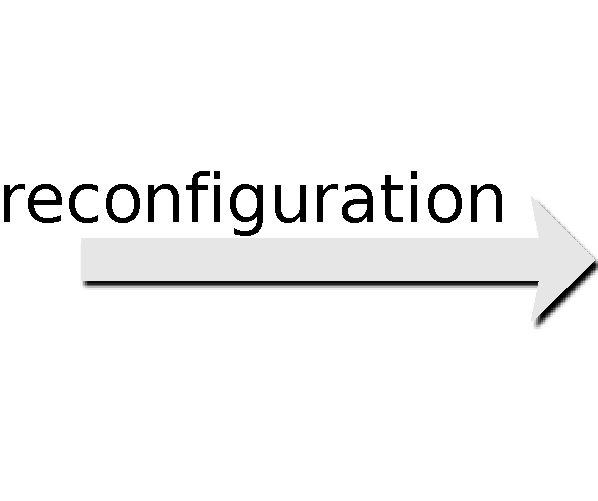
\includegraphics[width=2cm]{img/arrow_reconfiguration}
\end{minipage}
\begin{minipage}[b]{0.40\textwidth}
\begin{lstlisting}
N1: VM1 VM6
N2: VM2
N3: VM3 VM5
\end{lstlisting}
\end{minipage}
\caption{A reconfiguration motivated by \cstr{mostlySpread} constraints.}\label{fig: mostlySpread}
\end{reconfiguration}

\begin{itemize}

\item \cstr{mostlySpread(\{VM1, VM2, VM5\}, 2)}. This constraint was satisfied in the sour\-ce configuration as all the VM were running on  2 distinct servers. The constraint is still satisfied in the destination configuration as all the VMs are running on 3 distinct servers.

\item \cstr{mostlySpread(\{VM1,VM2\}, 1)}. This constraint was not satisfied in the source configuration as the VMs where running on \cstr{N1}. The relocation of \cstr{VM2} to \cstr{N3} fixed this violation.

\end{itemize}

\subsection{See also}

\subsubsection{Related Constraints}
\begin{itemize}
\item \cstrref{spread}: a constraint that guarantees the VMs will never overlap on a same server, even during the reconfiguration process.
\item \cstrref{lazySpread}: a constraint similar to \cstr{mostlySpread} but that guarantee every VMs are running on distinct servers.
\end{itemize}

\printListOfInheritance{mostlySpread}

\clearpage
% !TEX root =  ../main.tex
\section{Preserve}

\subsection{Definition} 

\subsubsection{Signature} \cstr{preserve(s : set<VM>, r:string, n : number)}

\begin{itemize}
\item \cstr{s}: a non-empty set of VMs for a meaningful constraint. VMs not in the \st{Running} state are ignored.
\item \cstr{r} : a resource identifier such as \cstr{mem}, \cstr{ucpu}, \cstr{pcpu} to identify the physical memory,
the computational capacity, the physical CPUs, respectively.
\item \cstr{n}: a positive amount of resources
\end{itemize}

The \cstr{preserve} constraint ensures each running VM in \cstr{s} is hosted on a server
having at minimum an amount of resource of type \cstr{r} equals to \cstr{n} dedicated to the VM.

\classification{preserve}{application administrator}{Resource allocation,VM placement}{VM-to-server placement,Resource management}

\subsubsection{Usage}

The \cstr{preserve} constraint allows to control the resource allocated to the given VMs.
This constraint may first be used inside a provisioning algorithm developed by an application administrator
to indicate to the resource manager an ideal amount of resources to provide to the VMs to let them work at a peak level of performance.
%

Inside a non-conservative consolidated environment, a server may host several VMs that currently
ask for a small amount of resources. In this situation, the server may become saturated if VMs ask suddenly for a little more resources. This situation is not idyllic as these micro variations may lead to numerous relocations. To prevent that situation and reduce the frequency of the reconfigurations, the datacenter administrator may use one \cstr{preserve} constraint to 
over-allocate a minimum amount of resources to the VMs that ask for a small amount of resources.

\subsubsection{Example}

Figure~\ref{fig: preserve} depicts a sample reconfiguration between a source and a destination configuration where each server provides 8 unit of CPU and 7 unit of memory resources to VMs. Each VM is associated to a gray rectangle that denotes its resource requirement, expressed using \cstr{preserve} constraints. A rectangle overlapping another one on a dimension indicates the two associated VMs have to share resources. This reveals an overloaded server. Figure~\ref{fig: preserve plan} depicts the associated event-based reconfiguration plan. The following \cstr{preserve} constraints were considered:

\begin{figure}[htb]
\centering
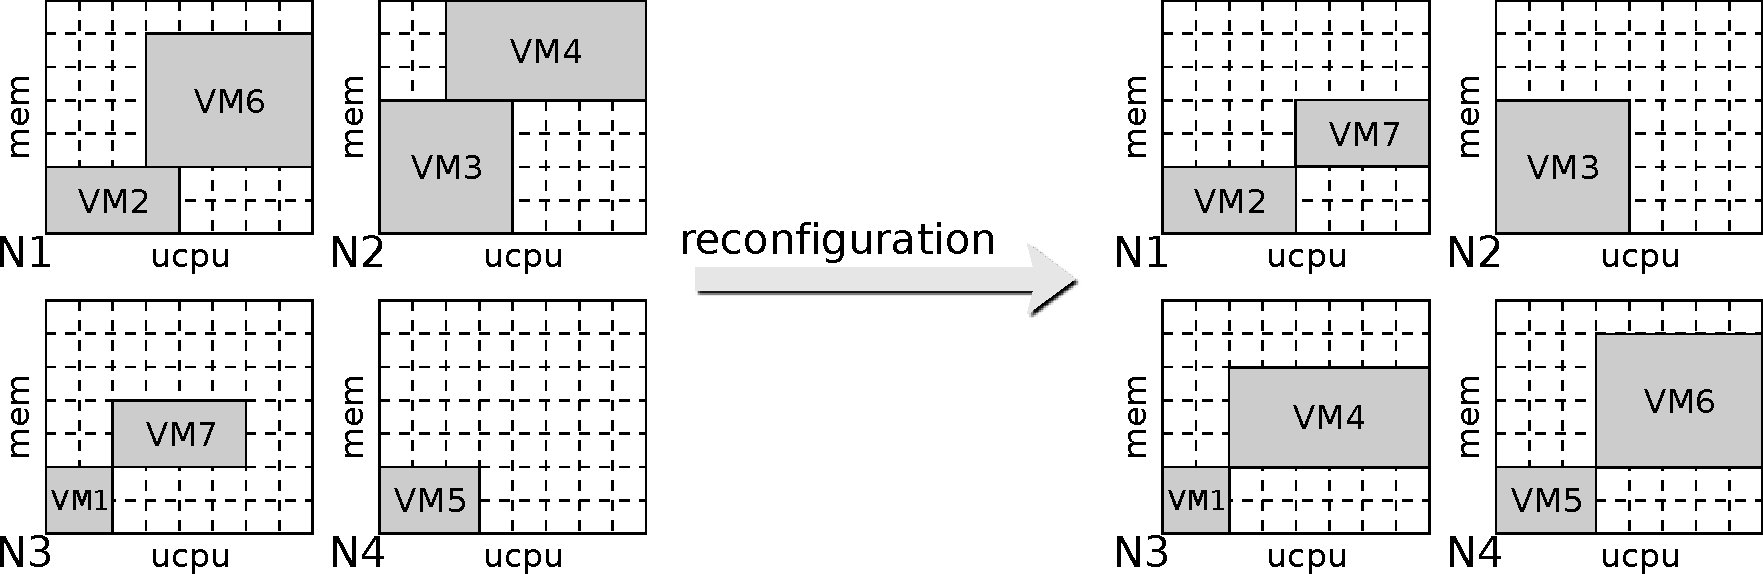
\includegraphics[width=\textwidth]{img/preserve}
\caption{A reconfiguration motivated by \cstr{preserve} constraints.}\label{fig: preserve}
\end{figure}


\begin{reconfPlan}
\centering
\begin{tabular}{ll}
\O & $\rightarrow$ relocate(VM6)\\
!relocate(VM6)\ & $\rightarrow$ relocate(VM7)\\
!relocate(VM7)\ & $\rightarrow$ relocate(VM4)
\end{tabular}
\caption{Event-based reconfiguration plan.}\label{fig: preserve plan}
\end{reconfPlan}


\begin{itemize}
\item \cstr{preserve(\{VM2, VM3\},4,"ucpu")}. This constraint was not satisfied in the source configuration as the
hosting servers of the given VMs do not provide enough resource to them: \cstr{N1} provides 8 unit of
CPU resources but \cstr{VM6} requires 5 units and \cstr{VM2} requires 4 units . In addition, VMs on \cstr{N2} required 10 units of CPU resources. These violation were fixed by relocating \cstr{VM4} and \cstr{VM6} to \cstr{N3} and \cstr{N4}, respectively.
%
However, \cstr{N4} does not initially provides enough resources to host simultaneously \cstr{VM4} and \cstr{VM7}. It has then be decided to relocate first \cstr{VM6} to \cstr{N4}�to liberate enough resource on \cstr{N1} to host \cstr{VM7}. Once this relocation terminated, enough resources were available on \cstr{N3} to
host \cstr{VM4}.

\item \cstr{preserve(\{VM1, VM7, VM5\},2,"mem")}. This constraint was satisfied in the source configuration as
their hosting servers provided enough memory resources to meet their requirement. The constraint is still
satisfied in the destination configuration despite the relocation of \cstr{VM7}.
\end{itemize}

\fullVersion{
\subsection{Model}
\label{preserve: model}
For each d-slice placement variable of the involved VMs,
its resource demand is modified to ask with at least the required amount of resources
if the demand was lesser than the amount to provide.
The constraint is modeled as follow:

\begin{equation*}
\begin{split}
\forall V \in \mathcal{V},\ preserve(V, n) & \triangleq\\
	& \forall v_i \in V, d_i^{cpu} = min(d_i^{cpu}, n)
\end{split}
\end{equation*}

\subsection{Violation Detection}

The detection of misplaced VMs can be made by observing the free resource on the current configuration. For each server, if the VM resource demand is greater than the server capacity then,
VMs will have to move. It is however not possible to check for the VMs that will be relocated in practice 
as this will be a technical choice depending on the global environment. A safe approach is then to consider that every VM on the server may have to be relocated.

\subsection{Availability}

\subsubsection{In {\btrp}}

The \cstr{preserve} constraint is available in {\btrp} since version 2.1. As the resource usage
of the d-slices placement variables is a constant, no specific Choco constraints are required.
Its model is then similar to the one detailed in~\ref{preserve: model}.
}
\subsection{See also}

\subsubsection{Related Constraints}
\begin{itemize}
\item \cstrref{oversubscription}: A constraint made available to the
datacenter administrator to control the resource overbooking on the servers. 
\end{itemize}

\printListOfInheritance{preserve}
\clearpage
% !TEX root =  ../main.tex
\section{Oversubscription}

\subsection{Definition}

\subsubsection{Signature} \cstr{oversubscription(s : set<server>, r : string, x : number)}

\begin{itemize}
\item \cstr{s} : a non-empty set of servers
\item \cstr{r} : a resource identifier such as \cstr{mem}, \cstr{ucpu}, \cstr{pcpu} to identify the physical memory,
the computational capacity, the physical CPUs, respectively.
\item \cstr{x} : a positive percentage
\end{itemize}

The \cstr{oversubscription} constraint ensures the online servers in \cstr{s} have for each hosted VM, 
an amount of free resources at least equals to a given factor of a physical resource.
Servers not in the \st{Online} state and VMs not in the \st{Running} state are ignored.

\classification{oversubscription}{datacenter administrator}{Resource allocation}{Resource management}

\subsubsection{Usage}

The memory is usually considered as the bottleneck that limitooor the servers hosting capacity.
Originally, the memory was not shareable between the VMs so their cumulated requirement shall not exceed the servers capacity. Hypervisors such as Xen~\cite{xen-memory-sharing} or VMWare~\cite{vmware-memory-sharing} now provide sharing systems to oversubscribe the memory. 
The datacenter administrator can then use \cstr{oversubscription} constraint to control this sharing. With a factor greater than 100\%,
a server can host simultaneously VMs with a cumulated memory usage that exceed its capacity. A high factor increases the hosting capabilities of the servers but may alter the VMs performance due to the overhead of the memory sharing system.

It is also accepted to oversubscribe the physical CPUs (PCPUs) of a server. Each VM uses one or more virtual CPUs (VCPUs) and for the maximum performance, each VCPU should be mapped to a dedicated PCPU. In practice, multiple VCPU are mapped to a same PCPU when the performance overhead is acceptable.
In 2010, The Virtual Management Index reported an oversubcription ratio of 200\%: each PCPU is allocated to 2 VCPUs on average.~\cite{vmi}

Finally, a VM is usually an instance of a given template that define the maximum amount of computational resources (UCPU) it can consume. To increase the hosting capacity of the servers, the resource are often allocated dynamically, on demand,
rather than statically\cite{pMapper,violin,bobroff2007dynamic,entropy-vee09}. It is however not desirable to place too many VMs that currently consume a few uCPU on a single server as it increases the chances of having a saturated server if the VMs simultaneously increase their uCPU demand. One solution to control this oversubscription is to ensure to each of the VMs a given percentage of its maximum uCPU resource usage. For example, the datacenter administrator may use one \cstr{oversubscription} constraint and an oversubscription ratio of 80\% to ensure each server must be able to provide each of the VMs it hosts 80\% of the VM's maximum uCPU usage, even if its current demand is inferior. 

\subsubsection{Example}

Figure~\ref{fig: oversubscription} depicts a sample reconfiguration between a source and a destination configuration where each server provides 8 unit of CPU and 7 unit of memory resources to VMs. The rectangles of the VMs denotes their maximum requirements while the grey part denotes their usage. During the reconfiguration, the following \cstr{oversubscription} constraints were considered:

\begin{figure}[htb]
\centering
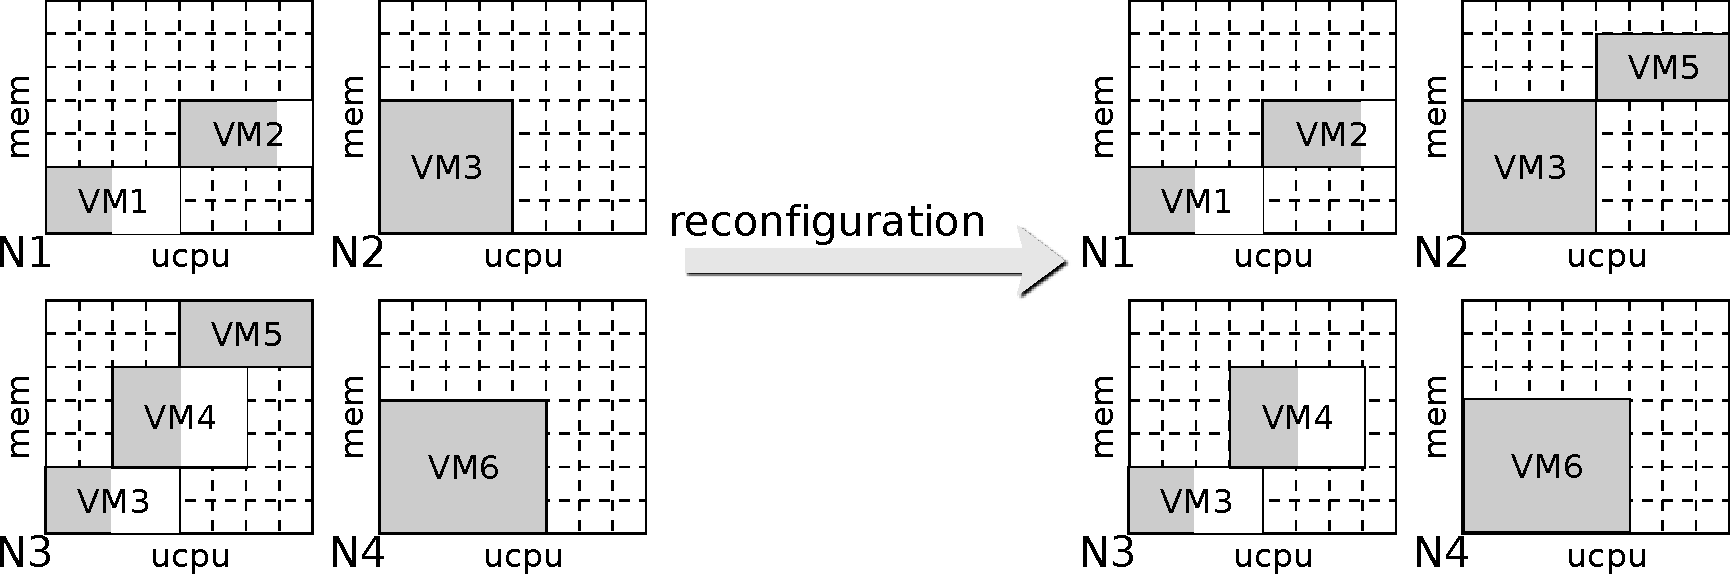
\includegraphics[width=\textwidth]{img/oversubscription}
\caption{A reconfiguration motivated by \cstr{oversubscription} constraints.}\label{fig: oversubscription}
\end{figure}


\begin{itemize}
\item \cstr{oversubscription(\{N1,N2\},"ucpu", 100\%)}. This constraint was satisfied in the source configuration
as each of the hosted VMs has enough UCPU resources to satisfy its maximum usage. The constraint is still
satisfied in the destination configuration despite the relocation of \cstr{VM5} to \cstr{N2}.

\item \cstr{oversubscription(\{N3, N4\},"ucpu",66\%)}. This constraint was not satisfied in the source configuration.
\cstr{VM3} and \cstr{VM4} were consuming 50\% of their maximum UCPU resources allowed but the presence
of \cstr{VM5} disallows them to be able to consume the required 66\%. The reconfiguration process
fixed that violation by relocating \cstr{VM5} to \cstr{N3}. As a result, \cstr{VM3} and \cstr{VM4} are ensured to be
able to consume at least 66\% of their maximum allowed. In practice, there will be able to consume 100\%.

\end{itemize}


\fullVersion{
\subsection{Model}

\subsection{Violation Detection}

\subsection{Availability}

\subsubsection{In {\btrp}}
}

\subsection{See also}

\subsubsection{Related Constraints}
\begin{itemize}
\item \cstrref{preserve}: A constraint to control the resource allocation
at the VM level.
\item \cstrref{singleCapacity}: A constraint to control the resource available on servers.
\end{itemize}

\printListOfInheritance{oversubscription}
\clearpage
% !TEX root =  ../main.tex
\section{CumulatedCapacity}

\subsection{Definition}

\subsubsection{Signature} \cstr{cumulatedCapacity(s:set<server>, r:string, nb:number)}

\begin{itemize}
\item \cstr{s}: a non-empty set of servers for a meaningful constraint. Servers not in the \st{Online} state are ignored.
\item \cstr{r} : a resource identifier such as \cstr{vm}, \cstr{mem}, \cstr{ucpu}, \cstr{pcpu} or \cstr{nodes} to identify the number of virtual machines, the physical memory, the computational capacity, the physical CPUs, respectively.
\item \cstr{nb}: a positive amount of resources. 
\end{itemize}

The \cstr{cumulatedCapacity} constraint restricts to a maximum of \cstr{nb}, the total amount
of a specific resource of type \cstr{r} that can be used on the online servers in \cstr{s} to run VMs.


\classification{cumulatedCapacity}{datacenter administrator}{VM placement,Resource allocation}{VM-to-server placement,Resource management}


\subsubsection{Usage}

The \cstr{cumulatedCapacity} constraint enables first the datacenter administrator to control 
the shared resources of
a platform. As an example, each VM has at least one IP address to be accessible from the network.
In practice, a datacenter has a finite pool of addresses to share among all the VMs.
Such a datacenter has then a global hosting capacity limited by the size of the address pool.
In this setting, one \cstr{cumulatedCapacity} constraint may be used to limit the hosting capacity
of VMs according to the size of the address pool.

The \cstr{cumulatedCapacity} constraint may also be used to control license restrictions.
As an example, on a datacenter running vSphere, the hosting capacity is limited by the cumulated amount of
memory allotted to the running VMs.~\cite{vsphere-license} In this setting, one \cstr{cumulatedCapacity}
constraint may be use by the datacenter administrator to guarantee the overall consumption of memory used
on the servers running VMWare is necessarily lesser to the maximum allowed by the acquired licenses.


\subsubsection{Example}

Figure~\ref{fig: cumulatedCapacity} depicts a sample reconfiguration between a source and a destination configuration where each server provides 8 unit of CPU and 7 unit of memory resources to VMs. Each VM is associated to a gray rectangle that denotes its resource usage. In this setting, the following \cstr{cumulatedCapacity} constraints were considered :

\begin{figure}[htb]
\centering
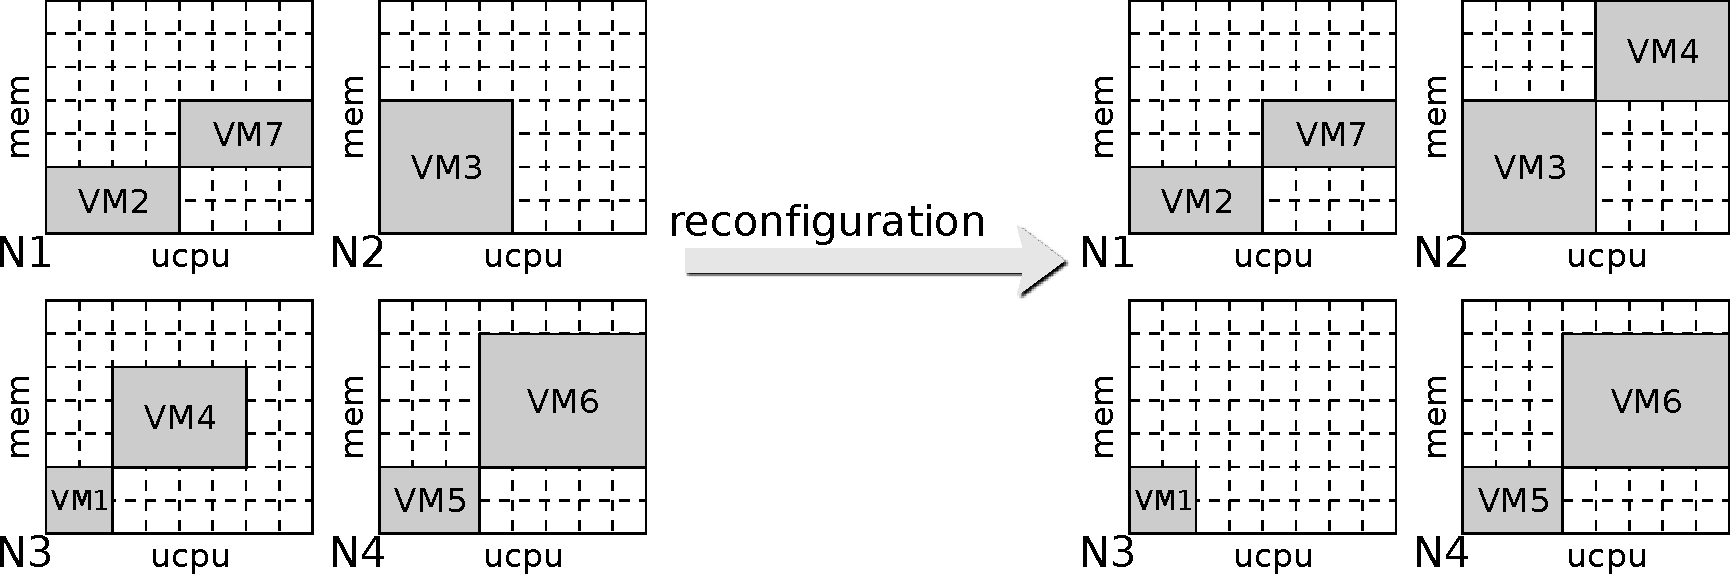
\includegraphics[width=\textwidth]{img/cumulatedCapacity}
\caption{A reconfiguration motivated by \cstr{cumulatedCapacity} constraints.}\label{fig: cumulatedCapacity}
\end{figure}


\begin{itemize}
\item \cstr{cumulatedCapacity(\{N1, N3\},7,"mem")}. This constraint was not satisfied in the source configuration as the cumulated memory usage on \cstr{N3} and \cstr{N1} was equals to 9.
This violation was fixed by relocating \cstr{VM4} to \cstr{N2}.

\item \cstr{cumulatedCapacity(\{N3, N4\},3,"vm")}. This constraint was not satisfied in the source configuration as there was
4 VMs running on the two nodes while the constraint restricts this number to 3 at maximum. This violation was fixed with the relocation of \cstr{VM4} to \cstr{N2}.

\item \cstr{cumulatedCapacity(\{N2, N4\},16,"ucpu")}. This constraint was satisfied in the source configuration as the cumulated UCPU usage of \cstr{N2} and \cstr{N4} was equals to 12. The constraint is still
satisfied in the destination configuration as the cumulated UCPU usage equals 16.
\end{itemize}


\fullVersion{
\subsection{Model}

This constraint is modeled by restricting the occurrences of d-slices hosted on the given servers.

\begin{equation*}
\begin{split}
\forall N \subseteq \mathcal{N},\ cumulatedCapacity(N, nb) \triangleq&\\
 & \forall v_i \in \mathcal{V},\ \sum_{d_i |�d_i^{host} \in n |�n \in {N}} d_i \leq nb
\end{split}
\end{equation*}

\subsection{Violation Detection}

The detection of the violating elements in \cstr{globalHostingCapacity} consists in counting VMs
that are hosted on the given server. When the amount of VMs is greater than the maximum
allowed, then the difference indicates the minimum number of VMs that are misplaced.
Such a detection is however not capable to indicate the VMs that are actually misplaced.


\subsection{Availability}

\subsubsection{In {\btrp}}

The constraint is available under the name \texttt{capacity} since version 2.1. The constraint is
modeled using one \emph{among}~\cite{among} constraint that directly counts the VMs assigned
to any server in the designated group of servers.

\begin{equation*}
\begin{split}
\forall N \subseteq \mathcal{N},\ globalHostingCapacity(N) \triangleq&\\
 & among(nb, \{ d_i^{host} | n_i \in N\}),
\end{split}
\end{equation*}
}
\subsection{See also}

\subsubsection{Related Constraints}
\begin{itemize}
\item \cstrref{singleCapacity}: A constraint to restrict the resource capacity on each server. A \cstr{cumulatedCapacity} constraint is then equivalent to a \cstr{single\-Capacity} constraint when the set of servers in \cstr{cumulatedCapacity} is a singleton.
\end{itemize}

\printListOfInheritance{cumulatedCapacity}
\clearpage
% !TEX root =  ../main.tex
\section{SingleCapacity}

\subsection{Definition}

\subsubsection{Signature} \cstr{singleCapacity(s:set<server>, nb:number, r:string)}

\begin{itemize}
\item \cstr{s}: a non-empty set of servers for a meaningful constraint. Servers not in the \st{Online}
state are ignored.
\item \cstr{r} : a resource identifier such as \cstr{mem}, \cstr{ucpu}, \cstr{pcpu} or \cstr{vm} to identify the physical memory,
the computational capacity, the physical CPUs or the number of hosted VMs, respectively.
\item \cstr{nb}: a positive amount of resources.
\end{itemize}


The \cstr{singleCapacity} constraint restricts to a maximum of \cstr{nb}, the amount
of a specific resource of type \cstr{r} that can be used on each of the online servers
in \cstr{s} to run VMs.

\classification{singleCapacity}{datacenter administrator}{VM placement,Resource allocation}{Resource management,VM-to-server placement}

\subsubsection{Usage}

The \cstr{singleCapacity} constraint is used by a datacenter administrator to indicate to the VM manager,
the practical amount of resources on each server, that will be available to the VMs.
As an example, a server having 4~GB of RAM running a Xen hypervisor~\cite{xen-sosp03} cannot offer this
amount of memory to the VMs as the \emph{Domain-0} requires memory resources to run. Using a \cstr{singleCapacity} constraint, the datacenter administrator may then declare the practical amount of memory that will be available to the VMs by removing the amount used by the \emph{Domain-0}.

Management operations, such as migrations, requires CPU resources on the involved servers.
When every resources are devoted to the running VMs, a migration will alter their performance as the hypervisor will use a significant amount of the resources that was allotted to the VMs, to manage the migration.
Using \cstr{singleCapacity} constraints, the datacenter administrator may prevent this temporary performance loss by dedicating in advance some resources to the hypervisor. Typically a core or a CPU, to let it perform the management operations without impacting the running VMs.

\subsubsection{Example}

Figure~\ref{fig: singleCapacity} depicts a sample reconfiguration between a source and a destination configuration where each server provides 8 unit of CPU and 7 unit of memory resources to VMs. Each VM is associated to a gray rectangle that denotes its resource usage. In this setting, the following \cstr{singleCapacity} constraints were considered :

\begin{figure}[htb]
\centering
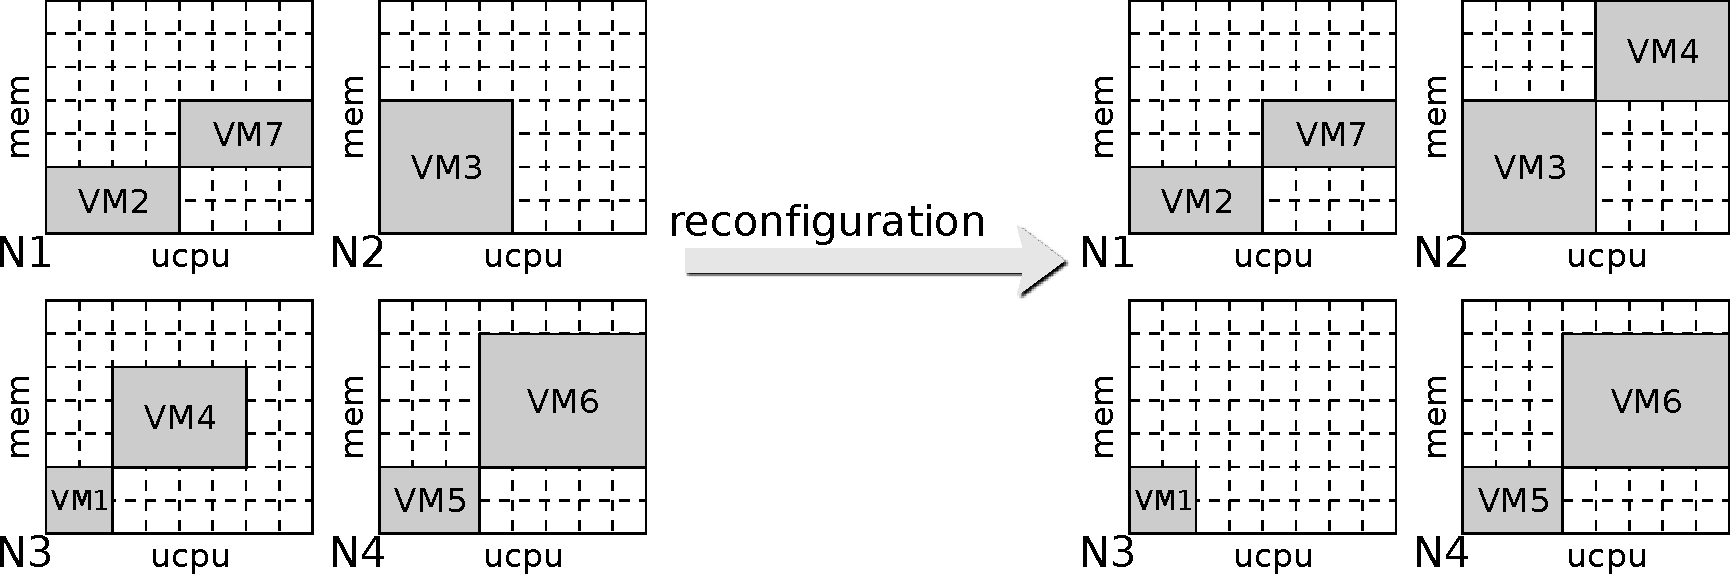
\includegraphics[width=\textwidth]{img/singleCapacity}
\caption{A reconfiguration motivated by \cstr{singleCapacity} constraints.}\label{fig: singleCapacity}
\end{figure}


\begin{itemize}
\item \cstr{singleCapacity(\{N1, N3\},4,"mem")}. This constraint was not satisfied in the source configuration
as the memory usage by the VMs on \cstr{N1} and \cstr{N3} equals 4 and 5, respectively.
This violation was fixed by relocating \cstr{VM4} to \cstr{N2} to liberate some resources.

\item \cstr{singleCapacity(\{N1, N2\},8,"ucpu")}. This constraint was satisfied in the source configuration
as the UCPU consumption of the running VMs was equals to 7 at maximum. The constraint is still satisfied
in the destination configuration as the relocation of \cstr{VM4} to \cstr{N2} makes the UCPU resource usage of \cstr{N2}
to 8, the maximum allowed.

\item \cstr{singleCapacity(\{N3\},1,"vm")}. This constraint was not satisfied in the source configuration
as the number of VMs running on \cstr{N3} was 2. The reconfiguration process fixed this violation by relocating
\cstr{VM4} to \cstr{N2}.
\end{itemize}

\fullVersion{
\subsection{Model}

\paragraph{Using the RP}

\subsection{Violation Detection}

The detection of the violating elements in \cstr{singleCapacity} consists in counting the VMs
that are hosted on each of the servers. When the amount of VMs exceed the maximum allowed, then
the difference indicates the minimum number of VMs that are misplaced. Such a detection is however
not capable to indicate the VMs that are actually misplaced.

\subsection{Availability}

\subsubsection{In BtrPlace}

Model depends on the content of \cstr{ns}. If it is a subset of the whole servers, then occurrence constraints. Otherwise, a bin packing constraint is preferable.
}

\subsection{See also}

\subsubsection{Related Constraints}
\begin{itemize}
\item \cstrref{cumulatedCapacity}: This constraint can be used when the resource restriction is related to the aggregation of some servers' resources.

\item \cstrref{preserve}: This constraint can be used in addition of \cstr{singleCapacity} constraint to ensure every VM has a sufficient amount of resources to run at peak level, according to the resources made available by \cstr{singleCapacity} constraints.

\end{itemize}

\emulatedWith{singleCapacity}{cumulatedCapacity}{\cstr{singleCapacity(ns, nb, r)}}{\cstr{\tforall n \tin ns, cumulatedCapacity(\{n\}, nb, r)}}
\printListOfInheritance{singleCapacity}
\clearpage
% !TEX root =  ../main.tex
\section{MinSpareResources}

\subsection{Definition}

\subsubsection{Signature} \cstr{minSpareResources(s : set<server>, rc : string, n : number)}

\begin{itemize}
\item \cstr{s} : a non-empty set of servers for a meaningful constraint.
\item \cstr{rc} : a resource identifier such as \cstr{mem}, \cstr{ucpu}, \cstr{pcpu} or \cstr{nodes} to identify the physical memory,
the computational capacity, the physical CPUs or the node itself, respectively.
\item \cstr{n} : a positive number
\end{itemize}

The \cstr{minSpareResources} restricts to at least \cstr{n}, the number of free resources directly
available for VMs on the online servers in \cstr{s}. Servers in the \st{Offline} state are ignored.

\classification{minSpareResources}{datacenter administrator}{Resource allocation}{Resource management,Power saving,Capacity planning}

\subsubsection{Usage}

This constraint deserves the control of a power saving strategy. The most effective solution
to reduce the energy consumption of a non-saturated datacenter is to turn off unused servers
and to turn them on and off depending on the load variation.
When a load spike arise, it may be a necessary to put some servers online to make their resources available to the VMs.~\cite{hermenier-xhpc06,vmware-dpm}
The time to boot the awaited servers may however be significant and alter the reactivity of the datacenter
when it faces an emergency situations. One solution is to let online a controlled number
of \emph{spare} resources that can be used instantly to absorb the load increase.
A datacenter administrator may then use  \cstr{minSpareResources} constraints
to control the minimum number of free resources to let directly available while the other unused resources are still manageable by the power saving strategy.

\subsubsection{Example}

Figure~\ref{fig: minSpareResources} depicts a sample reconfiguration between a source and a destination configuration where each server provides 8 unit of CPU and 7 unit of memory resources to VMs. During the reconfiguration, several relocations have been performed and the server \cstr{N3} has been turned off to save power. In this setting, the following \cstr{minSpareResources} constraints were considered:

\begin{figure}[htb]
\centering
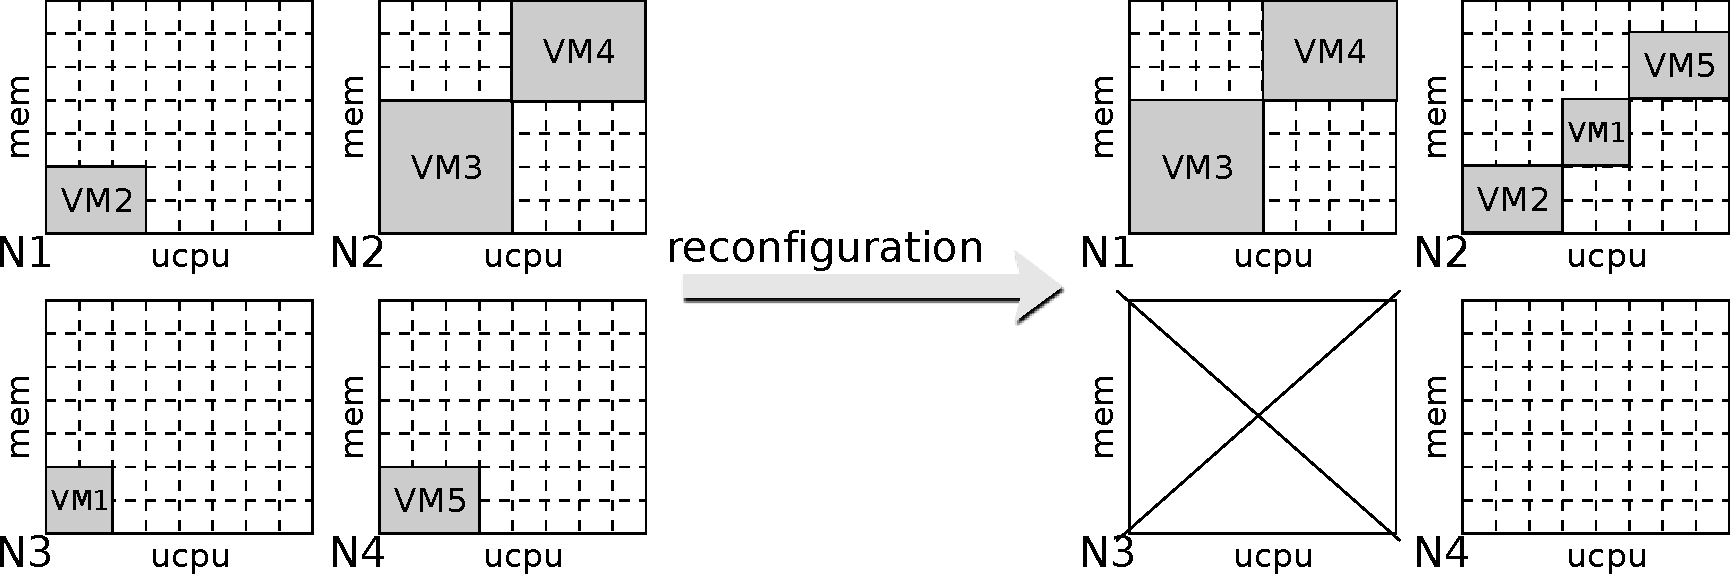
\includegraphics[width=\textwidth]{img/minSpareResources}
\caption{A reconfiguration motivated by \cstr{minSpareResources} constraints.}\label{fig: minSpareResources}
\end{figure}

\begin{itemize}

\item \cstr{minSpareResouces(\{N1,N2,N3\},"ucpu",0)}. This constraint was satisfied in the source configuration as 11 unit of CPU were directly available to the running VMs. The constraint is also satisfied in the destination configuration as 0 unit are available: resources on \cstr{N3} are not considered as it is in the \st{offline} state.

\item \cstr{minSpareResources(\{N2\},"mem",1)}. This constraint was not satisfied in the source configuration as no memory resources were available on \cstr{N2}. The reconfiguration process fixed that violation by relocating away \cstr{VM4} and \cstr{VM3} and host \cstr{VM2},\cstr{VM1}, and \cstr{VM5} while keeping one unity of memory resources directly available.

\item \cstr{minSpareResources(\{N2,N3,N4\},"node",1)}. This constraint was not satisfied in the source configuration as no servers were idle. The reconfiguration fixed this violation by relocating all the VMs on \cstr{N4} to other servers while keeping it in the \st{Online} state.

\end{itemize}

\fullVersion{
\subsection{Model}

The \cstr{noIdleOnlines} constraint is modeled in terms of the RPs variable by restricting
the state variable of each involved server to 0 depending on the number of VMs running
on the servers.

\begin{equation*}
\begin{split}
\forall N \in \mathcal{N},\ offline(N) & \triangleq\\
&	\forall n_i \in N, 
\sum_{d_i |�v_i \in \mathcal{V}} d_i = 0 \imply n_i^q = 0
\end{split}
\end{equation*}

\subsection{Violation detection}

To compute the list of violating elements, it is a necessary to check for each of 
the involved  server that are still online without running any VMs. This indicates
the violating servers.


\subsection{Availability}

\subsubsection{In {\btrp}}

The constraint is available in {\btrp} under the name \cstr{noIdleOnlines}.
To check whether a server is running a VM or not, we rely on the variable
indicating its memory usage. When this variable equals 0, then it is considered
the server does not host any VM and has to be turned off.

\begin{equation*}
\begin{split}
\forall N \in \mathcal{N},\ offline(N) & \triangleq\\
&	\forall n_i \in N,  eq(n_i^{mem}, 0) \imply eq(n_i^q, 0)
\end{split}
\end{equation*}
}

\subsection{See also}

\subsubsection{Related Constraints}
\begin{itemize}
\item \cstrref{maxSpareResources}: This constraint controls the maximum number of unused but available resources.
\end{itemize}


\printListOfInheritance{minSpareResources}
%
%\begin{itemize}
%\item \hyperref[cstr: offline]{\cstr{offline}}: The turn off servers in any condition.
%\end{itemize}
\clearpage
% !TEX root =  ../main.tex
\section{MaxSpareResources}

\subsection{Definition}

\subsubsection{Signature} \cstr{maxSpareResources(s : set<server>, rc : string, n : number)}

\begin{itemize}
\item \cstr{s} : a non-empty set of servers for a meaningful constraint.
\item \cstr{rc} : a resource identifier such as \cstr{mem}, \cstr{ucpu}, \cstr{pcpu} or \cstr{nodes} to identify the physical memory,
the computational capacity, the physical CPUs or the node itself, respectively.
\item \cstr{n} : a positive number
\end{itemize}

The \cstr{maxSpareResources} restricts to at most \cstr{n}, the number of free resources directly
available for VMs on the online servers in \cstr{s}. Servers in the \st{Offline} state are ignored.


\classification{maxSpareResources}{datacenter administrator}{Resource allocation}{Resource management,Power saving,Capacity planning}

\subsubsection{Usage}

This constraint deserves a power saving concern. 
The most effective solution to reduce the energy consumption of a non-saturated datacenter is to turn off unused servers and to turn on and off servers depending on the load variation.
When a load spike arise, it may then be a necessary to put some servers online to make their resources available to the VMs.~\cite{hermenier-xhpc06,vmware-dpm}
The time to boot the awaited servers may however be significant and alter the reactivity of the datacenter
when it faces an emergency situations. One solution is to let online a controlled number
of \emph{spare} resources that can be used instantly to absorb the load increase.
A datacenter administrator may then use one \cstr{maxSpareResources} constraint
to control the maximum number of unused servers to let online while the others will
be turned off to save power.

It is worth noting that despite this constraint is applicable to a various number of resources, it is preferable to only focus
the \cstr{nodes} resource. Indeed, a server provides resources at a coarse grain and it may not be possible to manage the resources according to the constraint by only managing the servers state.

\subsubsection{Example}

Figure~\ref{fig: maxSpareResources} depicts a sample reconfiguration between a source and a destination configuration where each server provides 8 unit of CPU and 7 unit of memory resources to VMs. During the reconfiguration, several relocations have been performed and the server \cstr{N3} has been turned off to save power. In this setting, the following \cstr{maxSpareResources} constraints were considered:

\begin{figure}[htb]
\centering
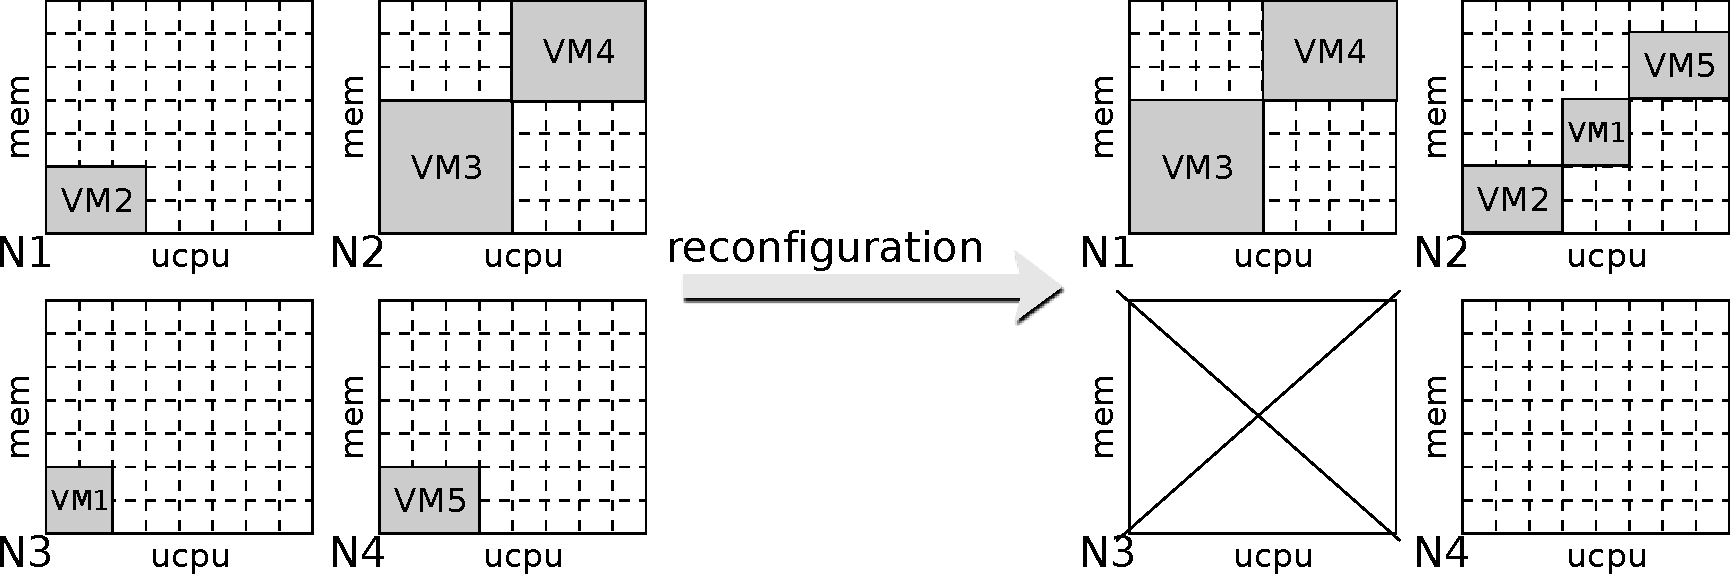
\includegraphics[width=\textwidth]{img/maxSpareResources}
\caption{A reconfiguration motivated by \cstr{maxSpareResources} constraints.}\label{fig: maxSpareResources}
\end{figure}


\begin{itemize}

\item \cstr{maxSpareResources(\{N2,N3,N4\},"node",1)}. This constraint was satisfied in the source configuration as no server was idle. The constraint is still satisfied in the destination configuration as only \cstr{N4} is in the \st{Online} state and idle.

\item \cstr{maxSpareResources(\{N1,N2,N3\},"ucpu",10)}. This constraint was not satisfied in the source configuration
as 11 uCPU was directly available to the running VMs. The reconfiguration fixed this violation. With the shutdown of \cstr{N3},
8 uCPU resources are directly available in the destination configuration, which is an amount allowed by the constraint.

\item \cstr{maxSpareResources(\{N1, N3\},"mem",3)}. This constraint was not satisfied in the source configuration
as 10 unit of memory were directly available to the running VMs. The reconfiguration fixed this violation. With the shutdown of \cstr{N3}, and the saturation of \cstr{N1}, no memory resources are left available to the VMs on these servers.

\end{itemize}

\fullVersion{
\subsection{Model}

The \cstr{noIdleOnlines} constraint is modeled in terms of the RPs variable by restricting
the state variable of each involved server to 0 depending on the number of VMs running
on the servers.

\begin{equation*}
\begin{split}
\forall N \in \mathcal{N},\ offline(N) & \triangleq\\
&	\forall n_i \in N, 
\sum_{d_i |�v_i \in \mathcal{V}} d_i = 0 \imply n_i^q = 0
\end{split}
\end{equation*}

\subsection{Violation detection}

To compute the list of violating elements, it is a necessary to check for each of 
the involved  server that are still online without running any VMs. This indicates
the violating servers.


\subsection{Availability}

\subsubsection{In {\btrp}}

The constraint is available in {\btrp} under the name \cstr{noIdleOnlines}.
To check whether a server is running a VM or not, we rely on the variable
indicating its memory usage. When this variable equals 0, then it is considered
the server does not host any VM and has to be turned off.

\begin{equation*}
\begin{split}
\forall N \in \mathcal{N},\ offline(N) & \triangleq\\
&	\forall n_i \in N,  eq(n_i^{mem}, 0) \imply eq(n_i^q, 0)
\end{split}
\end{equation*}
}

\subsection{See also}

\subsubsection{Related Constraints}
\begin{itemize}
\item \cstrref{minSpareResources}: This constraint restricts the number of unused online servers to a given minimum.
\end{itemize}

\printListOfInheritance{maxSpareResources}
%
%\begin{itemize}
%\item \hyperref[cstr: offline]{\cstr{offline}}: The turn off servers in any condition.
%\end{itemize}
\clearpage
% !TEX root =  ../main.tex
\section{MaxOnlines}

\subsection{Definition}

\subsubsection{Signature} \cstr{maxOnlines(s : set<server>, n : number)}

\begin{itemize}
\item \cstr{s} : a non-empty set of servers for a meaningful constraint.
\item \cstr{n} : a positive number, inferior to the number of servers in \cstr{s}.
\end{itemize}


The \cstr{maxOnlines} ensures the number of online servers in \cstr{s} is inferior or equals to \cstr{n}.

\classification{maxOnlines}{datacenter administrator}{Resource allocation}{Resource management,Power saving,Capacity planning}

\subsubsection{Usage}

This constraint deserves the control of the datacenter hosting capacity. A datacenter may
be composed of servers that differ in their hardware capacity or performance.
It may however not be possible to keep all the servers online simultaneously. As an example,
the cooling system or the power distribution unit may restrict the number of online servers due to its delivering capacity.
Licenses restrictions, such as the per-server license model of XenServer, may also limits the number of nodes that are online
simultaneously.~\cite{xen-server}

In this setting, once the maximum number of online servers reached,  turning on one additional server
to use its specificities is only allowed if an online server can be turned off in exchange.
In this setting, a datacenter administrator may then use of \cstr{maxOnlines} constraints to control the number of online servers and automatically manage their state if needed.

\subsubsection{Example}

Figure~\ref{fig: maxOnlines} depicts a sample reconfiguration between a source and a destination configuration where only servers \cstr{N1}, \cstr{N2} and \cstr{N3} are online in the source configuration.
Each VM is associated to a gray rectangle that denotes its resource usage in terms of memory and UCPU.
In the source configuration, the server \cstr{N1} was saturated has \cstr{VM4} and \cstr{VM6} were competing for the same resources. The reconfiguration process fixed this violation but also consider the following \cstr{maxOnlines} constraints:

\begin{figure}[htb]
\centering
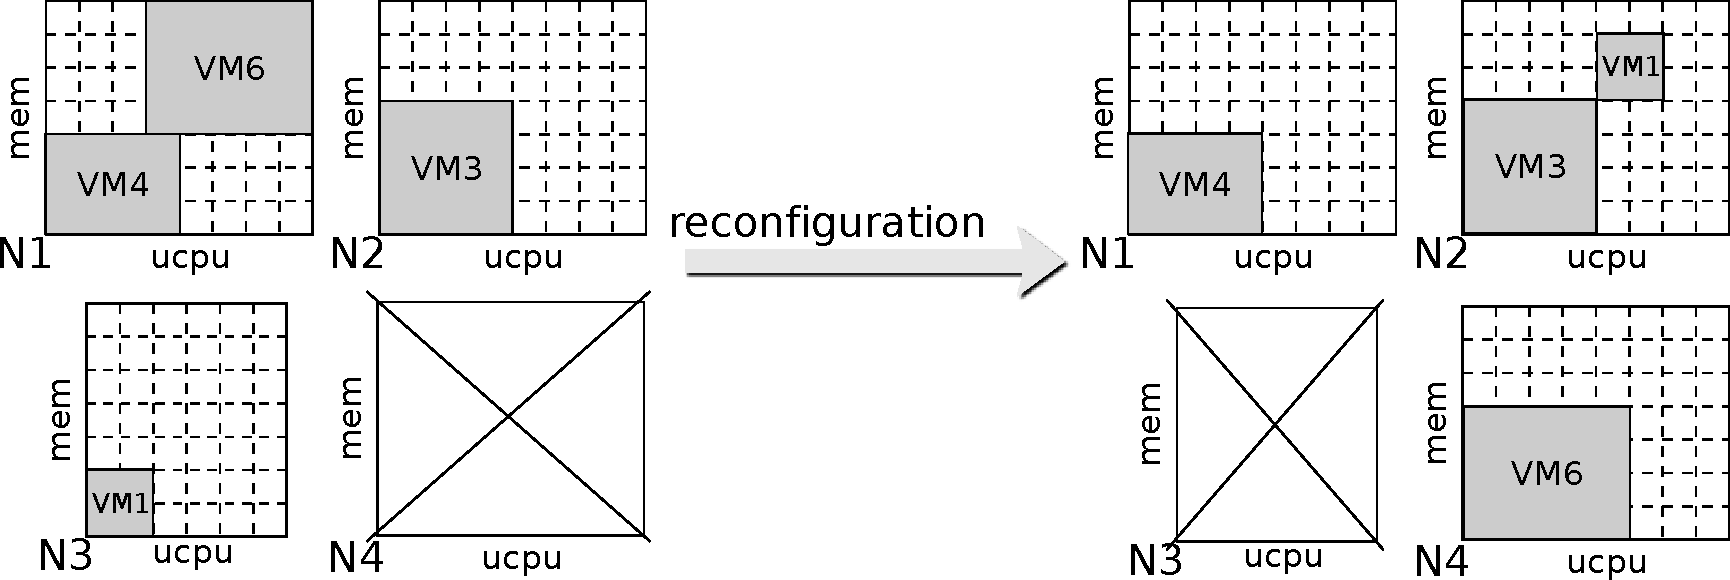
\includegraphics[width=\textwidth]{img/maxOnlines}
\caption{A reconfiguration motivated by \cstr{maxOnlines} constraints.}\label{fig: maxOnlines}
\end{figure}


\begin{itemize}

\item \cstr{maxOnlines(\{N1,N2, N3, N4\}, 3)}. This constraint was satisfied in the source configuration as three over the four
servers were in the \st{Online} state. The constraint is still satisfied in the destination configuration. \cstr{N4}�has been turned
on to host 	\cstr{VM6} but \cstr{N3} has been turned off in exchange according to the constraint specification. To be able to turned
off \cstr{N3}, \cstr{VM1} has been relocated to \cstr{N2}. Figure~\ref{fig: maxOnlines plan} depicts the associated event-based reconfiguration plan.

\begin{reconfPlan}[htb]
\centering
\begin{tabular}{ll}
\O & $\rightarrow$ relocate(VM1) \\
!relocate(VM1)\ & $\rightarrow$ halt(N3)\\
!halt(N3)\ & $\rightarrow$ boot(N4)\\
!boot(N4) & $\rightarrow$ relocate(VM6)
\end{tabular}
\caption{Event-based reconfiguration plan associated to the reconfiguration depicted in Figure~\ref{fig: maxOnlines}.}\label{fig: maxOnlines plan}
\end{reconfPlan}

\item \cstr{maxOnlines(\{N1, N3\},1)}. This constraint was not satisfied in the source configuration as the two servers were in the \st{Online}�state. The reconfiguration process fixed this violation by turning off \cstr{N3}.
\end{itemize}


\subsection{See also}

\subsubsection{Related Constraints}

\begin{itemize}
\item \cstrref{maxSpareResources}: A constraint to restrict the number of unused but available resources to a given maximum.
\end{itemize}


\printListOfInheritance{maxOnlines}

\clearpage
% !TEX root =  ../main.tex
\section{Offline}

\subsection{Definition}

\subsubsection{Signature} \cstr{offline(s : set<server>)}

The \cstr{offline} constraint forces every server in \cstr{s} to be set in the \st{Offline} state.

\subsubsection{Usage}

This constraint deserves first hardware maintenance concerns. Using this constraint, one datacenter administrator can turn off a set of servers to perform maintenance operation on the hardware

\classification{offline}{datacenter administrator}{Servers state}{Resource management}

\subsubsection{Example}

\fullVersion{
\subsection{Model}

The \cstr{offline} constraint is modeled in terms of the RPs variable by restricting
the state variable of each involved server to 0.

\begin{equation*}
\begin{split}
\forall N \in \mathcal{N},\ offline(N) & \triangleq\\
&	\forall n_i \in N, n_i^q = 0
\end{split}
\end{equation*}

\subsection{Violation detection}

To compute the list of violating elements, it is a necessary to check for each of 
the involved  server that are still online. VMs hosted on that server, including 
VMs in the \st{running}, the \st{paused}, and the \st{sleeping} states, have to be
relocated. This detection is optimal.

\subsection{Availability}

\subsubsection{In {\btrp}}

The constraint is available in {\btrp} under the name \cstr{offline}. It is
modeled by instantiated the state variable of each involved server to 1:

\begin{equation*}
\begin{split}
\forall N \in \mathcal{N},\ offline(N) & \triangleq\\
&	\forall n_i \in N, eq(n_i^q, 0)
\end{split}
\end{equation*}
}

\subsection{See also}
\subsubsection{Related constraints}
\begin{itemize}
\item \cstrref{online}: The opposite constraint that is used to force servers to being set in the \st{Online} state.
\item \cstrref{maxOnlines}:  To restrict the maximum number of servers that are simultaneously in the \st{Online} state.
\end{itemize}
\clearpage
% !TEX root =  ../main.tex
\section{Online}

\subsection{Definition}

\subsubsection{Signature} \cstr{online(s : set<server>)}

The \cstr{online} constraint forces every server in \cstr{s} to be set in the \st{Online} state.

\subsubsection{Usage}

This constraint deserves first the necessity of having servers available to host VMs.
This constraint is also useful in a context where servers can not be managed, \ie turned off.

\classification{online}{datacenter administrator}{Servers state}{Resource management}

\subsubsection{Example}

\fullVersion{
\subsection{Model}

The \cstr{online} constraint is modeled in terms of the RPs variable by restricting
the state variable of each involved server to 1.

\begin{equation*}
\begin{split}
\forall N \in \mathcal{N},\ online(N) & \triangleq\\
&	\forall n_i \in N, n_i^q = 1
\end{split}
\end{equation*}

\subsection{Violation detection}

To compute the list of violating elements, it is a necessary to check for each of 
the involved  server that are still offline. This detection is optimal.

\subsection{Availability}

\subsubsection{In {\btrp}}

The constraint is available in {\btrp} under the name \cstr{offline}. It is
modeled by instantiated the state variable of each involved server to 0:

\begin{equation*}
\begin{split}
\forall N \in \mathcal{N},\ online(N) & \triangleq\\
&	\forall n_i \in N, eq(n_i^q, 1)
\end{split}
\end{equation*}
}

\subsection{See also}
\subsubsection{Related constraints}
\begin{itemize}
\item \cstrref{offline}: The opposite constraint that is used to force servers to being set in the \st{Offline} state.
\end{itemize}

\printListOfInheritance{online}

\clearpage

%% !TEX root =  ../main.tex
\section{BorderPatrol}

\subsection{Definition}

The \cstr{root} constraint forces each running VM in s to not move from its current location. Non-running
VMs are ignored.

\classification{borderPatrol}{datacenter administrator}{VM placement, actions schedule}{reconfiguration}

\subsection{Usage}

\fullVersion{
\subsection{Model}

\subsection{Implementation using Btrplace}

\subsubsection{Modeling using Btrplace and Choco}

\subsubsection{Availability}

This constraint in available in Entropy since version 2.0 as "Root". The implementation
is fully compatible with the root constraint specification presented here.
}

\subsection{See also}
%\clearpage
%\input{constraints/globalOverSubscription}
%\clearpage
%% !TEX root =  ../main.tex
\section{GlobalSpareCapacity}

\subsection{Definition}

The \cstr{root} constraint forces each running VM in s to not move from its current location. Non-running
VMs are ignored.

\subsection{Usage}

\fullVersion{
\subsection{Model}

\subsection{Implementation using Btrplace}

\subsubsection{Modeling using Btrplace and Choco}

\subsubsection{Availability}

This constraint in available in Entropy since version 2.0 as "Root". The implementation
is fully compatible with the root constraint specification presented here.
}
\subsection{See also}
%\clearpage
%% !TEX root =  ../main.tex
\section{Platform}

\subsection{Definition}

The \cstr{root} constraint forces each running VM in s to not move from its current location. Non-running
VMs are ignored.

\subsection{Usage}

\fullVersion{
\subsection{Model}

\subsection{Implementation using Btrplace}

\subsubsection{Modeling using Btrplace and Choco}

\subsubsection{Availability}

This constraint in available in Entropy since version 2.0 as "Root". The implementation
is fully compatible with the root constraint specification presented here.
}

\subsection{See also}
%\clearpage
%% !TEX root =  ../main.tex
\section{Reconfigurable}

\subsection{Definition}

The \cstr{root} constraint forces each running VM in s to not move from its current location. Non-running
VMs are ignored.

\subsection{Usage}

\fullVersion{
\subsection{Model}

\subsection{Implementation using Btrplace}

\subsubsection{Modeling using Btrplace and Choco}

\subsubsection{Availability}

This constraint in available in Entropy since version 2.0 as "Root". The implementation
is fully compatible with the root constraint specification presented here.
}

\subsection{See also}
%\clearpage
%% !TEX root =  ../main.tex
\section{Running}

\subsection{Definition}

The \cstr{root} constraint forces each running VM in s to not move from its current location. Non-running
VMs are ignored.

\subsection{Usage}

\fullVersion{
\subsection{Model}

\subsection{Implementation using Btrplace}

\subsubsection{Modeling using Btrplace and Choco}

\subsubsection{Availability}

This constraint in available in Entropy since version 2.0 as "Root". The implementation
is fully compatible with the root constraint specification presented here.
}
\subsection{See also}
%\clearpage
%% !TEX root =  ../main.tex
\section{SingleSpareCapacity}

\subsection{Definition}

The \cstr{root} constraint forces each running VM in s to not move from its current location. Non-running
VMs are ignored.

\subsection{Usage}

\fullVersion{
\subsection{Model}

\subsection{Implementation using Btrplace}

\subsubsection{Modeling using Btrplace and Choco}

\subsubsection{Availability}

This constraint in available in Entropy since version 2.0 as "Root". The implementation
is fully compatible with the root constraint specification presented here.
}
\subsection{See also}
%\clearpage
%% !TEX root =  ../main.tex
\section{Sleeping}

\subsection{Definition}

The \cstr{root} constraint forces each running VM in s to not move from its current location. Non-running
VMs are ignored.

\subsection{Usage}

\fullVersion{
\subsection{Model}

\subsection{Implementation using Btrplace}

\subsubsection{Modeling using Btrplace and Choco}

\subsubsection{Availability}

This constraint in available in Entropy since version 2.0 as "Root". The implementation
is fully compatible with the root constraint specification presented here.
}

\subsection{See also}
%\clearpage
%% !TEX root =  ../main.tex
\section{Terminating}

\subsection{Definition}

The \cstr{root} constraint forces each running VM in s to not move from its current location. Non-running
VMs are ignored.

\subsection{Usage}

\subsection{Model}

\subsection{Implementation using Btrplace}

\subsubsection{Modeling using Btrplace and Choco}

\subsubsection{Availability}

This constraint in available in Entropy since version 2.0 as "Root". The implementation
is fully compatible with the root constraint specification presented here.

\subsection{See also}
%\clearpage
%% !TEX root =  ../main.tex
\section{Waiting}

\subsection{Definition}

The \cstr{root} constraint forces each running VM in s to not move from its current location. Non-running
VMs are ignored.

\subsection{Usage}

\subsection{Model}

\subsection{Implementation using Btrplace}

\subsubsection{Modeling using Btrplace and Choco}

\subsubsection{Availability}

This constraint in available in Entropy since version 2.0 as "Root". The implementation
is fully compatible with the root constraint specification presented here.

\subsection{See also}